\subsection{Interpretation of flatness in terms of relations}

Throughout this no. A denotes a ring, E a right A-module and F a left A-module.

Every element of \(\mathbf{E} \otimes_{\mathbf{A}} \mathbf{F}\) can be written in at least one way in the form \(z = \sum_{i=1}^{n} e_i \otimes f_i\) where \(e_i \in \mathbf{E}\) and \(f_i \in \mathbf{F}\) . The following lemma gives a condition under which this sum is zero:

LEMMA 10. Let \((f_{\lambda})_{\lambda \in \mathbf{L}}\) be a family of generators of \(\mathbf{F}\) and \((e_{\lambda})_{\lambda \in \mathbf{L}}\) a family of elements of \(\mathbf{E}\) of finite support. For \(\sum_{\lambda \in \mathbf{L}} e_{\lambda} \otimes f_{\lambda} = 0\) , it is necessary and sufficient that there exist a finite set \(\mathbf{J}\) , a family \((x_{j})_{j \in \mathbf{J}}\) of elements of \(\mathbf{E}\) and a family \((a_{j\lambda})\) ( \(j \in \mathbf{J}, \lambda \in \mathbf{L}\) ) of elements of \(\mathbf{A}\) with the following properties:

\begin{enumerate}
\def\labelenumi{(\arabic{enumi})}
\item
  the family \((a_{j\lambda})\) has finite support;
\item
  \(\sum_{\lambda \in L} a_{j\lambda} f_{\lambda} = 0\) for all \(j \in J\) ;
\item
  \(e_{\lambda} = \sum_{j\in J}x_ja_{j\lambda}\) for all \(\lambda \in \mathbf{L}\) .
\end{enumerate}

Loosely speaking, the system of \(e_{\lambda}\) must be a linear combination with coefficients in E of systems of elements of A which are ``relations between the \(f_{\lambda}\) ''.

Consider the free A-module \(\mathrm{A}_{s}^{(\mathrm{L})}\) , its canonical basis \((u_{\lambda})\) and the homomorphism \(g: \mathrm{A}_{s}^{(\mathrm{L})} \to \mathrm{F}\) such that \(g(u_{\lambda}) = f_{\lambda}\) for all \(\lambda \in L\) ; denoting by R the kernel of g, we have (since the \(f_{\lambda}\) generate F) an exact sequence

\[
\mathrm{R} \xrightarrow {i} \mathrm{A} _ {s} ^ {(L)} \xrightarrow {g} \mathrm{F} \longrightarrow 0
\]

where i denotes the canonical injection. By Lemma 1 of no. 1 we derive the exact sequence

\[
\mathrm{E} \otimes_ {\mathrm{A}} \mathrm{R} \xrightarrow {1 \otimes i} \mathrm{E} \otimes_ {\mathrm{A}} \mathrm{A} _ {s} ^ {(L)} \xrightarrow {1 \otimes g} \mathrm{E} \otimes_ {\mathrm{A}} \mathrm{F} \longrightarrow 0.\tag{13}
\]

Now, \(\mathbf{E} \otimes_{\mathbf{A}} \mathbf{A}_{s}^{(L)}\) is canonically identified with \(\mathbf{E}^{(L)}\) , a family \(e = (e_{\lambda}) \in \mathbf{E}^{(L)}\) being identified with \(\sum_{\lambda \in L} e_{\lambda} \otimes u_{\lambda}\) (Algebra, Chapter II, § 3, no. 7, Corollary 1 to Proposition 7). For such a family to belong to the kernel of \(1_{\mathbf{E}} \otimes g\) , it is necessary and sufficient that \(\sum_{\lambda \in L} e_{\lambda} \otimes f_{\lambda} = 0\) in \(\mathbf{E} \otimes_{\mathbf{A}} \mathbf{F}\) ; taking account of the exact sequence (13), this is equivalent to saying that \(e\) belongs to the image of \(1_{\mathbf{E}} \otimes i\) , in other words there is a relation of the form

\[
\sum_ {\lambda \in L} e _ {\lambda} \otimes u _ {\lambda} = \sum_ {j \in J} x _ {j} \otimes i (r _ {j})\tag{14}
\]

where \(x_{j} \in \mathbf{E}\) , \(r_{j} \in \mathbf{R}\) and \(\mathbf{J}\) is finite. Writing \(i(r_{j}) = \sum_{\lambda \in \mathbf{L}} a_{j\lambda} u_{\lambda}\) , the hypothesis \(r_{j} \in \mathbf{R}\) implies the relation \(\sum_{\lambda \in \mathbf{L}} a_{j\lambda} f_{\lambda} = 0\) for all \(j \in \mathbf{J}\) ; on the other hand the relation (14) implies \(e_{\lambda} = \sum_{j \in J} x_{j} a_{j\lambda}\) for all \(\lambda \in \mathbf{L}\) (Algebra, Chapter II, § 3, no. 7, Corollary 1 to Proposition 7), which completes the proof.

PROPOSITION 13. For E to be F-flat (no. 2, Definition 1), it is necessary and sufficient that the following condition be satisfied:

\begin{enumerate}
\def\labelenumi{(\Alph{enumi})}
\setcounter{enumi}{17}
\tightlist
\item
  If \((e_i)_{i \in I}\) and \((f_i)_{i \in I}\) are two finite families of elements of E and F respectively such that \(\sum_{i \in I} e_i \otimes f_i = 0\) in E \(\otimes_{\mathbf{A}} \mathbf{F}\) , there exists a finite set J, a family \((x_j)_{j \in J}\) of elements of E and a family \((a_{jl})\) ( \(j \in J\) , \(i \in I\) ) of elements of A, with the following properties:
\end{enumerate}

\begin{enumerate}
\def\labelenumi{(\arabic{enumi})}
\item
  \(\sum_{i\in I}a_{ji}f_i = 0\) for all \(j\in J\)
\item
  \(e_i = \sum_{j \in J} x_j a_{ji}\) for all \(i \in I\) .
\end{enumerate}

Suppose that E is F-flat. Let \((e_{i})\) and \((f_{i})\) be finite families of elements such that \(\sum_{i\in I}e_{i}\otimes f_{i}=0\) in \(E\otimes_{A}F\) , and let \(F'\) be the submodule of F generated by the \(f_{i}\) . Since the canonical mapping \(E\otimes_{A}F'\to E\otimes_{A}F\) is injective, we have also \(\sum_{i\in I}e_{i}\otimes f_{i}=0\) in \(E\otimes_{A}F'\) and Lemma 10 can then be applied to E and \(F'\) ; thus families \((x_{j})\) and \((a_{ji})\) are obtained satisfying the conditions of (R).

Conversely, suppose that condition (R) holds. Let \(\mathbf{F}'\) be a submodule of \(\mathbf{F}\) and let \(y = \sum_{i\in I}e_i\otimes f_i\) be an element of the kernel of the canonical mapping \(\mathbf{E}\otimes_{\mathbf{A}}\mathbf{F}'\to \mathbf{E}\otimes_{\mathbf{A}}\mathbf{F}\) . Since (R) holds, there exist families \((x_j)\) and \((a_{jl})\) satisfying conditions (1) and (2). We conclude that, in \(\mathbf{E}\otimes_{\mathbf{A}}\mathbf{F}'\) ,

\[
y = \sum_ {i, j} x _ {j} a _ {j i} \otimes f _ {i} = \sum_ {j \in J} (x _ {j} \otimes \sum_ {i \in I} a _ {j i} f _ {i}) = 0.
\]

Hence \(\mathbf{E} \otimes_{\mathbf{A}} \mathbf{F}' \to \mathbf{E} \otimes_{\mathbf{A}} \mathbf{F}\) is injective.

COROLLARY 1. For a right A-module E to be flat, it is necessary and sufficient that the following condition hold:

(RP) If \((e_i)_{i\in I}\) and \((b_i)_{i\in I}\) are two finite families of elements of E and A respectively such that \(\sum_{i\in I}e_i b_i = 0\) , there exists a finite set J, a family \((x_j)_{j\in J}\) of elements of E and a family \((a_{ji})\) ( \(j\in J\) , \(i\in I\) ) of elements of A such that \(\sum_{i\in I}a_{ji}b_i = 0\) for all \(j\in J\) and \(e_i = \sum_{j\in J}x_j a_{ji}\) for all \(i\in I\) .

Condition (RP) is just condition (R) of Proposition 13 applied to the module \(\mathbf{F} = \mathbf{A}_s\) .

Loosely speaking, (RP) states: every ``relation'' between the \(b_{i}\) , with coefficients in E, is a linear combination (with coefficients in E) of ``relations'' between the \(b_{i}\) with coefficients in A.

Let us consider in particular a homomorphism of A to a ring B, which makes B into a right A-module. We know (no. 3, Proposition 1) that this is equivalent to saying that this A-module is flat, or that it is flat for every left A-module \(A_{s}^{m}\) ( \(m \geqslant 1\) ). Applying condition (R) of Proposition 13 with E = B and \(F = A_{s}^{m}\) we obtain the following condition:

COROLLARY 2. For the ring B to be a flat right A-module, it is necessary and sufficient that it satisfy the following condition:

(RP') Every solution \((y_{k})_{1\leqslant k\leqslant n}\) , consisting of elements of B, of a system of homogeneous linear equations

\[
\sum_ {k = 1} ^ {n} y _ {k} c _ {k l} = 0 \quad (1 \leqslant i \leqslant m)\tag{15}
\]

with coefficients \(c_{kl}\) in A, is a linear combination

\[
y _ {k} = \sum_ {j = 1} ^ {q} b _ {j} z _ {j k} \quad (1 \leqslant k \leqslant n)\tag{16}
\]

with coefficients \(b_{j} \in \mathbf{B}\) , of solutions \((z_{jk})_{1 \leqslant k \leqslant n}\) of the system (15), consisting of elements \(z_{jk}\) of \(\mathbf{A}\) .

\section{FAITHFULLY FLAT MODULES}

\subsection{Definition of faithfully flat modules}

PROPOSITION 1. Let E be a right A-module. The following four properties are equivalent:

\begin{enumerate}
\def\labelenumi{(\alph{enumi})}
\tightlist
\item
  For a sequence \(\mathbf{N}' \xrightarrow{v} \mathbf{N} \xrightarrow{w} \mathbf{N}''\) of left A-modules to be exact, it is necessary and sufficient that the sequence
\end{enumerate}

\[
\mathrm{E} \otimes_ {\mathrm{A}} \mathrm{N} ^ {\prime} \xrightarrow {1 \otimes v} \mathrm{E} \otimes_ {\mathrm{A}} \mathrm{N} \xrightarrow {1 \otimes w} \mathrm{E} \otimes_ {\mathrm{A}} \mathrm{N} ^ {\prime \prime}
\]

be exact.

\begin{enumerate}
\def\labelenumi{(\alph{enumi})}
\setcounter{enumi}{1}
\item
  E is flat and, for every left A-module N, the relation \(E \otimes_{A} N = 0\) implies N = 0.
\item
  E is flat and, for every homomorphism \(v: \mathbf{N}' \to \mathbf{N}\) of left A-modules, the relation \(\mathbf{1}_{\mathbf{E}} \otimes v = 0\) implies \(v = 0\) .
\item
  E is flat and, for every maximal left ideal m of A, \(E \neq Em\) . To simplify the writing we set \(T(Q) = E \otimes_{A} Q\) for every left A-module Q and \(T(v) = 1_{E} \otimes v\) for every homomorphism v of left A-modules.
\end{enumerate}

We prove first the equivalence of (a), (b) and (c).

We prove that (a) implies (b). If (a) holds, clearly E is flat (§ 2, no. 3, Proposition 1). On the other hand, let N be a left A-module such that T(N) = 0 and consider the sequence 0 → N → 0; the hypothesis T(N) = 0 means that the sequence 0 → T(N) → 0 is exact. By (a) the sequence 0 → N → 0 is exact, whence N = 0.

We show that (b) implies (c). Suppose that (b) holds and let \(v: \mathbf{N}' \to \mathbf{N}\) be a homomorphism and \(\mathbf{I}\) its image. As the image of \(\mathrm{T}(v)\) is identified with \(\mathrm{T}(\mathbf{I})\) (§ 2, no. 3, Remark 2), the hypothesis \(\mathrm{T}(v) = 0\) implies \(\mathrm{T}(\mathbf{I}) = 0\) , hence \(\mathbf{I} = 0\) by (b) and consequently \(v = 0\) .

We show that (c) implies (a). Suppose then that (c) holds and consider a sequence

\[
\mathrm{N} ^ {\prime} \xrightarrow {v} \mathrm{N} \xrightarrow {w} \mathrm{N} ^ {\prime \prime}\tag{1}
\]

of homomorphisms of left A-modules and the corresponding sequence

\[
\mathrm{T} \left(\mathrm{N} ^ {\prime}\right) \xrightarrow {\mathrm{T} (v)} \mathrm{T} (\mathrm{N}) \xrightarrow {\mathrm{T} (w)} \mathrm{T} \left(\mathrm{N} ^ {\prime \prime}\right).\tag{2}
\]

If the sequence (1) is exact, so is (2), since E is flat (§ 2, no. 3, Proposition 1). Conversely, if (2) is exact, we have first \(\mathbf{T}(w \circ v) = \mathbf{T}(w) \circ \mathbf{T}(v) = 0\) , hence \(w \circ v = 0\) by hypothesis. Set \(\mathbf{I} = v(\mathbf{N}')\) and \(\mathbf{K} = \overline{w}^{-1}(0)\) ; then I is contained in K by the above. Consider the exact sequence

\[
0 \longrightarrow \mathrm{I} \stackrel {i} {\longrightarrow} \mathrm{K} \stackrel {p} {\longrightarrow} \mathrm{K} / \mathrm{I} \longrightarrow 0
\]

i and p being the canonical mappings. As E is flat, the sequence

\[
0 \longrightarrow \mathrm{T} (\mathrm{I}) \xrightarrow {\mathrm{T} (i)} \mathrm{T} (\mathrm{K}) \xrightarrow {\mathrm{T} (p)} \mathrm{T} (\mathrm{K} / \mathrm{I}) \longrightarrow 0
\]

is exact, in other words, T(K/I) is isomorphic to T(K)/T(I), which is 0 by hypothesis, since T(I) (resp. T(K)) is identified with the image of T(v) (resp. the kernel of T(w)) (§ 2, no. 3, Remark 2). But the relation T(p) = 0 implies p = 0 by hypothesis, hence K = I, which proves that the sequence (1) is exact.

Finally we show the equivalence of (b) and (d). If (b) holds, then

\[
\mathrm{E} / \mathrm{Em} = \mathrm{E} \otimes_ {\mathbf {A}} (\mathrm{A} _ {s} / \mathfrak {m}) \neq 0
\]

since \(A_{s}/m \neq 0\) ; whence (d). Conversely, suppose that (d) holds; every left ideal \(a \neq A\) of A is contained in a maximal left ideal m (Algebra, Chapter I, §8, no. 7, Theorem 2), then the hypothesis \(E \neq Em\) implies \(E \neq Ea\) , in other words, \(E \otimes_{A} (A_{s}/a) \neq 0\) . That is to say, for every monogenous left A-module \(N \neq 0\) , \(T(N) \neq 0\) . If now N is any left A-module \(\neq 0\) , it contains a monogenous submodule \(N' \neq 0\) ; since E is flat, \(T(N')\) is identified with a subgroup of \(T(N)\) ; we have just seen that \(T(N') \neq 0\) , hence \(T(N) \neq 0\) .

DEFINITION 1. A right A-module E is called faithfully flat if it satisfies the four equivalent conditions of Proposition 1.

Faithfully flat left A-modules are defined similarly; clearly, for a left A-module E to be faithfully flat, it is necessary and sufficient that E, considered as a right \(A^{0}\) -module, be faithfully flat.

Remark. If E is a faithfully flat A-module, E is a faithful A-module: for, if an element \(a \in A\) is such that xa = 0 for all \(x \in E\) , the homothety \(h: b \mapsto ba\) in A is such that \(1_{E} \otimes h = 0\) ; whence h = 0 by property (c) of Proposition 1, that is a = 0 since A has a unit element.

\textbf{Examples}\par

\begin{enumerate}
\def\labelenumi{(\arabic{enumi})}
\item
  The direct sum of a flat module and faithfully flat module is a faithfully flat module by virtue of property (d) of Proposition 1 and § 2, no. 3, Proposition 2.
\item
  As \(A_{s}\) is faithfully flat by virtue of criterion (d) of Proposition 1 and §2, no. 4, Example 1, it follows from (1) that every free module not reduced to 0 is faithfully flat. On the other hand, there exist non-zero direct factors of free modules (in other words, non-zero projective modules) which are faithful but not faithfully flat (Exercise 2).
\item
  Let A be a principal ideal domain. For an A-module E to be faithfully flat, it is necessary and sufficient that it be torsion-free and \(E \neq Ep\) for every irreducible element (Algebra, Chapter VII, §1, no. 3) p of A; this follows immediately from §2, no. 4, Proposition 3 and criterion (d) of Proposition 1.
\end{enumerate}

\pandocbounded{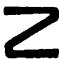
\includegraphics[keepaspectratio]{images/part001_f9c264f7.jpg}}

\begin{enumerate}
\def\labelenumi{(\arabic{enumi})}
\setcounter{enumi}{3}
\tightlist
\item
  Example (3) shows that the \(\mathbf{Z}\) -module \(\mathbf{Q}\) is a flat and faithful module, but not faithfully flat.
\end{enumerate}

PROPOSITION 2. Let E be a faithfully flat right A-module and \(u: \mathbf{N}' \to \mathbf{N}\) a left A-module homomorphism. For \(u\) to be injective (resp. surjective, bijective), it is necessary and sufficient that \(1_{\mathbf{E}} \otimes u: \mathbf{E} \otimes_{\mathbf{A}} \mathbf{N}' \to \mathbf{E} \otimes_{\mathbf{A}} \mathbf{N}\) be so.

This is an immediate consequence of criterion (a) of Proposition 1.

PROPOSITION 3. Let \(0 \to E' \to E \to E'' \to 0\) be an exact sequence of right A-modules. Suppose that \(E'\) and \(E''\) are flat and that one of them is faithfully flat. Then \(E\) is faithfully flat.

We know already that E is flat (§ 2, no. 5, Proposition 5). We verify that E has property (b) of Proposition 1. Let N be a left A-module. As E'' is flat, there is an exact sequence

\[
0 \rightarrow \mathrm{E} ^ {\prime} \otimes_ {\mathrm{A}} \mathrm{N} \rightarrow \mathrm{E} \otimes_ {\mathrm{A}} \mathrm{N} \rightarrow \mathrm{E} ^ {\prime \prime} \otimes_ {\mathrm{A}} \mathrm{N} \rightarrow 0
\]

(§ 2, no. 5, Proposition 4). If \(\mathbf{E} \otimes_{\mathbf{A}} \mathbf{N} = 0\) , it follows that \(\mathbf{E}' \otimes_{\mathbf{A}} \mathbf{N}\) and \(\mathbf{E}'' \otimes_{\mathbf{A}} \mathbf{N}\) are zero; as one of the modules \(\mathbf{E}', \mathbf{E}''\) is faithfully flat, this implies that \(\mathbf{N} = 0\) .

\subsection{Tensor products of faithfully flat modules}

PROPOSITION 4. Let R, S be two rings, E a right R-module and F an (R, S)-bimodule. Suppose that E is faithfully flat. Then, for F to be a flat (resp. faithfully flat) S-module, it is necessary and sufficient that \(E \otimes_{R} F\) be so.

\begin{enumerate}
\def\labelenumi{(\arabic{enumi})}
\item
  If \(\mathbf{F}\) is flat, \(\mathbf{E} \otimes_{\mathbb{R}} \mathbf{F}\) is flat ( \(\S 2\) , no. 7, Proposition 8).
\item
  Suppose that \(\mathbf{E} \otimes_{\mathbb{R}} \mathbf{F}\) is flat and let \(v: \mathbf{N}' \to \mathbf{N}\) be an injective left S-module homomorphism. The homomorphism
\end{enumerate}

\[
  \mathbf {1} _ {\mathbf {E}} \otimes \mathbf {1} _ {\mathbf {F}} \otimes v: \mathbf {E} \otimes_ {\mathbf {R}} \mathbf {F} \otimes_ {\mathbf {S}} \mathbf {N} ^ {\prime} \rightarrow \mathbf {E} \otimes_ {\mathbf {R}} \mathbf {F} \otimes_ {\mathbf {S}} \mathbf {N}
\]

is then injective (§ 2, no. 3, Proposition 1). It follows from Proposition 2 of no. 1 that \(\mathbf{1}_{\mathbf{F}} \otimes v \colon \mathbf{F} \otimes_{\mathbf{S}} \mathbf{N}' \to \mathbf{F} \otimes_{\mathbf{S}} \mathbf{N}\) is injective; then \(\mathbf{F}\) is a flat S-module (§ 2, no. 3, Proposition 1).

\begin{enumerate}
\def\labelenumi{(\arabic{enumi})}
\setcounter{enumi}{2}
\item
  Suppose that F is faithfully flat and let N be a left S-module such that \(E \otimes_{R} F \otimes_{S} N = 0\) . Since E is faithfully flat, this implies that \(F \otimes_{S} N = 0\) , whence N = 0 since F is faithfully flat; this proves that \(E \otimes_{R} F\) is faithfully flat.
\item
  Suppose that \(E \otimes_{R} F\) is faithfully flat and let N be a left S-module such that \(F \otimes_{S} N = 0\) . Then \(E \otimes_{R} F \otimes_{S} N = 0\) , whence N = 0, which shows that F is faithfully flat.
\end{enumerate}

COROLLARY. Let C be a commutative ring and E and F two faithfully flat C-modules. Then the C-module \(E \otimes_{C} F\) is faithfully flat.

Apply Proposition 4 with \(\mathbf{R} = \mathbf{S} = \mathbf{C}\) .

\subsection{Change of ring}

PROPOSITION 5. Let \(\rho\) be a homomorphism from a ring A to a ring B. If E is a faithfully flat right A-module, the right B-module \(\rho^{*}(\mathbf{E}) = \mathbf{E}_{(\mathbf{B})} = \mathbf{E} \otimes_{\mathbf{A}} \mathbf{B}\) is faithfully flat.

Apply Proposition 4 of no. 2 with R = A, S = F = B, noting that the B-module \(B_{d}\) is faithfully flat.

COROLLARY. If E is a faithfully flat right A-module and if a is a two-sided ideal of A, the right (A/a)-module E/Ea is faithfully flat.

Apply Proposition 5 with B = A/a, \(\rho\) being the canonical homomorphism.

PROPOSITION 6. Let A be a commutative ring, B an algebra over A and \(\rho: a \mapsto a . 1\) the canonical homomorphism of A to B. Suppose that B is a faithfully flat A-module. Then, for an A-module E to be flat (resp. faithfully flat), it is necessary and sufficient that the right B-module \(\mathrm{E}_{(\mathrm{B})} = \mathrm{E} \otimes_{\mathrm{A}} \mathrm{B}\) be flat (resp. faithfully flat).

\begin{enumerate}
\def\labelenumi{(\arabic{enumi})}
\item
  If E is flat (resp. faithfully flat), \(E_{(B)}\) is flat (resp. faithfully flat) by § 2, no. 7, Corollary 2 to Proposition 8 (resp. by Proposition 5).
\item
  Suppose that \(E_{(B)}\) is flat and let \(v: N' \to N\) be an injective A-module homomorphism. By § 2, no. 7, Corollary 3, the A-module \(E \otimes_{A} B\) is flat, hence the homomorphism \(1_{E} \otimes 1_{B} \otimes v: E \otimes_{A} B \otimes_{A} N' \to E \otimes_{A} B \otimes_{A} N\) is injective. As the right and left A-module structures on B coincide, this homomorphism is identified with
\end{enumerate}

\[
\mathrm{1} _ {\mathbf {E}} \otimes v \otimes \mathrm{1} _ {\mathbf {B}}: \mathrm{E} \otimes_ {\mathbf {A}} \mathrm{N} ^ {\prime} \otimes_ {\mathbf {A}} \mathrm{B} \rightarrow \mathrm{E} \otimes_ {\mathbf {A}} \mathrm{N} \otimes_ {\mathbf {A}} \mathrm{B}.
\]

As B is a faithfully flat A-module, it follows that \(1_{E} \otimes v: E \otimes_{A} N' \to E \otimes_{A} N\) is injective (no. 1, Proposition 2), which shows that E is flat.

\begin{enumerate}
\def\labelenumi{(\arabic{enumi})}
\setcounter{enumi}{2}
\tightlist
\item
  Suppose finally that \(E_{(B)}\) is faithfully flat. First of all E is flat by (2). Also let N be an A-module such that \(E \otimes_{A} N = 0\) . Then \(E \otimes_{A} N \otimes_{A} B = 0\) , whence, since the right and left A-module structures on B coincide, \(E \otimes_{A} B \otimes_{A} N = 0\) , which may also be written ( \(E \otimes_{A} B\) ) \(\otimes_{B} (B \otimes_{A} N) = 0\) . As \(E_{(B)}\) is a faithfully flat B-module, this implies that \(B \otimes_{A} N = 0\) (no. 1, Proposition 1), whence N = 0 since B is a faithfully flat A-module (no. 1, Proposition 1).
\end{enumerate}

\subsection{Restriction of scalars}

PROPOSITION 7. Let A, B be two rings and \(\rho\) a homomorphism of A to B. Let E be a faithfully flat right B-module. For \(\rho^{*}(\mathrm{E})\) to be a flat (resp. faithfully flat) right A-module, it is necessary and sufficient that B be a flat (resp. faithfully flat) right A-module.

Applying Proposition 4 of no. 2 with B, A, E, B in place of R, S, E, F respectively, and the right A-module structure on B being defined by \(\rho\) , it is seen that

B is a flat (resp. faithfully flat) A-module if and only if \(E \otimes_{B} B = \rho^{*}(E)\) is a flat (resp. faithfully flat) A-module.

\textbf{Remarks}\par

\begin{enumerate}
\def\labelenumi{(\arabic{enumi})}
\item
  Proposition 7 shows that, for B to be a faithfully flat A-module, it is sufficient that there exist one faithfully flat B-module which is also a faithfully flat A-module.
\item
  Let A, B, C be three rings and \(\rho: A \rightarrow B\) , \(\sigma: B \rightarrow C\) two ring homomorphisms. Proposition 7 shows that if C is a faithfully flat B-module and B a faithfully flat A-module, then C is a faithfully flat A-module. If C is a faithfully flat B-module and a faithfully flat A-module, then B is a faithfully flat A-module (taking the modules as right modules, to fix the ideas). On the other hand B and C may be faithfully flat A-modules without C being a faithfully flat B-module (Exercise 7).
\end{enumerate}

\subsection{Faithfully flat rings}

PROPOSITION 8. Let A, B be two rings and \(\rho\) a homomorphism from A to B. Suppose that there exists a right B-module E such that \(\rho_{*}(E)\) is a faithfully flat A-module. Then:

\begin{enumerate}
\def\labelenumi{(\roman{enumi})}
\item
  For every left A-module F, the canonical homomorphism \(j: \mathbf{F} \to \mathbf{F}_{(\mathbf{B})} = \mathbf{B} \otimes_{\mathbf{A}} \mathbf{F}\) (such that \(j(x) = 1 \otimes x\) for all \(x \in \mathbf{F}\) ) is injective.
\item
  For every left ideal \(\mathfrak{a}\) of \(\mathbf{A},\overline{\rho}^{-1}(\mathbf{Ba}) = \mathfrak{a}\) .
\item
  The homomorphism \(\rho\) is injective.
\item
  For every maximal left ideal \(\mathfrak{m}\) of A, there exists a maximal left ideal \(\mathfrak{n}\) of B such that \(\overline{\rho}^{-1}(\mathfrak{n}) = \mathfrak{m}\) .
\end{enumerate}

We prove (i). We know (Algebra, Chapter II, § 5, no. 2, Corollary to Proposition 5) that for every right B-module M, the canonical A-homomorphism \(i: \mathbf{M} \to \rho_*(\mathbf{M}) \otimes_{\mathbf{A}} \mathbf{B} = \rho^*(\rho_*(\mathbf{M}))\) defined by \(i(y) = y \otimes 1\) is injective and that the A-module \(i(\mathbf{M})\) is a direct factor of \(\rho_*(\mathbf{M}) \otimes_{\mathbf{A}} \mathbf{B}\) . Hence, for every left A-module F,

\[
i \otimes 1 _ {F}: \rho_ {*} (M) \otimes_ {A} F \rightarrow \rho_ {*} (M) \otimes_ {A} B \otimes_ {A} F
\]

is injective (§ 2, no. 1, Lemma 2). Taking \(\mathbf{M} = \mathbf{E}\) , it follows (since \(i \otimes 1_{\mathbf{F}} = 1_{\mathbf{M}} \otimes j\) ) that \(j\) is injective (no. 1, Proposition 2).

Assertion (ii) follows from (i) by taking \(\mathbf{F} = \mathbf{A}_s / \mathfrak{a}\) and (iii) from (ii) by taking \(\mathfrak{a} = \{0\}\) .

Finally, if \(\mathfrak{m}\) is a maximal left ideal of \(\mathbf{A}\) , then \(\bar{\rho}^{-1}(\mathbf{B}\mathfrak{m}) = \mathfrak{m}\) by (ii), and consequently \(\mathbf{B}\mathfrak{m} \neq \mathbf{B}\) . Then there exists a maximal left ideal \(\mathfrak{n}\) of \(\mathbf{B}\) containing \(\mathbf{B}\mathfrak{m}\) (Algebra, Chapter I, § 8, no. 7, Theorem 2); then \(\mathfrak{m} \subset \bar{\rho}^{-1}(\mathfrak{n})\) and as \(\rho(1) \notin \mathfrak{n}\) , \(1 \notin \bar{\rho}^{-1}(\mathfrak{n})\) . Consequently \(\bar{\rho}^{-1}(\mathfrak{n}) = \mathfrak{m}\) .

If A and B satisfy the conditions of Proposition 8, A is usually identified with a subring of B by means of \(\rho\) .

COROLLARY. Under the hypotheses of Proposition 8, if B is left Noetherian (resp. Artinian), so is A.

If \((\mathfrak{a}_n)\) is a non-stationary increasing (resp. decreasing) sequence of left ideals of A, the sequence \((\mathrm{Ba}_n)\) of ideals of B is non-stationary and increasing (resp. decreasing) since \(\overline{\rho}^{-1}(\mathrm{Ba}_n) = \mathfrak{a}_n\) , contrary to the hypothesis.

*Remark (1). If A and B are commutative, we shall see in Chapter II, § 2, no. 5, Corollary 4 to Proposition 11, that the hypothesis of Proposition 8 implies that

for every \(\text{prime}\) ideal \(\mathfrak{p}\) of \(\mathbf{A}\) , there exists a \(\text{prime}\) ideal \(\mathfrak{q}\) of \(\mathbf{B}\) such that \(\overline{\rho}^{-1}(\mathfrak{q}) = \mathfrak{p}\) (where \(\mathfrak{p} = \mathbf{A} \cap \mathfrak{q}\) when \(\mathbf{A}\) is identified with a subring of \(\mathbf{B}\) ).*

An important application of Proposition 8 is when B is itself a faithfully flat A-module. But in this case we have the following more precise proposition:

PROPOSITION 9. Let A, B be two rings and \(\rho\) a homomorphism of A to B. The following five properties are equivalent:

\begin{enumerate}
\def\labelenumi{(\alph{enumi})}
\item
  The right A-module B is faithfully flat.
\item
  The homomorphism \(\rho\) is injective and the right A-module \(\mathbf{B} / \rho (\mathbf{A})\) is flat.
\item
  The right A-module B is flat and, for every left A-module F, the canonical homomorphism \(x \mapsto 1 \otimes x\) of F to B \(\otimes_{A} F\) is injective.
\item
  The right A-module B is flat and, for every left ideal a of A, \(\overline{\rho}^{-1}(\mathbf{B}\mathfrak{a}) = \mathfrak{a}\) .
\item
  The right A-module B is flat and, for every maximal left ideal m of A, there
\end{enumerate}

exists a maximal left ideal n of B such that \(\bar{\rho}^{-1}(\mathfrak{n}) = \mathfrak{m}\) .

By Proposition 8, (a) implies each of the properties (c), (d), (e). On the other hand, if (e) holds, then \(\mathbf{Bm} \neq \mathbf{B}\) for every maximal left ideal \(m\) of A (since there exists a maximal left ideal \(n\) of B such that \(\mathbf{Bm} \subset n\) ), and B is a faithfully flat A-module by criterion (d) of Proposition 1 of no. 1; hence (e) implies (a).

We shall now prove that \((c) \Rightarrow (d) \Rightarrow (b) \Rightarrow (a)\) , which will complete the proof. In the first place, (c) implies (d) by taking \(F = A_{s}/a\) in (c). If (d) holds, by taking \(a = \{0\}\) it follows that \(\rho\) is injective; (d) and §2, no. 6, Corollary to Proposition 7 imply that \(B/\rho(A)\) is a flat right A-module, that is (d) implies (b). Finally, if (b) holds, Proposition 3 of no. 1 applied to the exact sequence

\[
0 \longrightarrow \mathrm{A} _ {d} \stackrel {\rho} {\longrightarrow} \mathrm{B} \longrightarrow \mathrm{B} / \rho (\mathrm{A}) \longrightarrow 0
\]

shows that B is a faithfully flat right A-module, since \(A_{d}\) is faithfully flat.

*Remark (2). If A and B are commutative, we shall see in Chapter II, § 2 no. 5, Corollary 4 to Proposition 11 that the conditions of Proposition 9 are equivalent to the following:

\begin{enumerate}
\def\labelenumi{(\alph{enumi})}
\setcounter{enumi}{5}
\tightlist
\item
  B is a flat A-module and, for every prime ideal p of A, there exists an ideal q of B such that \(\overline{\rho}^{-1}(\mathfrak{q}) = \mathfrak{p}\) .
\end{enumerate}

Under the conditions of Proposition 9, let us identify A with a subring of B by means of \(\rho\) . The relation \(\bar{\rho}^{-1}(\mathbf{Ba}) = a\) then reads \(\mathbf{A} \cap \mathbf{Ba} = a\) . On the other hand if F is a left A-module, F is identified with its image in \(\mathbf{B} \otimes_{\mathbf{A}} \mathbf{F}\) under the canonical mapping \(x \mapsto 1 \otimes x\) ; if X is an additive subgroup of F, then we denote by BX the left sub-B-module of \(\mathbf{B} \otimes_{\mathbf{A}} \mathbf{F}\) generated by X. With this notation, we have:

PROPOSITION 10. Let B be a ring and A a subring of B such that B is a faithfully flat right A-module. Let F be a left A-module, F', F'' two submodules of F. Then:

\begin{enumerate}
\def\labelenumi{(\roman{enumi})}
\item
  The canonical mapping \(\mathbf{B} \otimes_{\mathbf{A}} \mathbf{F}' \to \mathbf{B} \otimes_{\mathbf{A}} \mathbf{F}\) is an isomorphism of \(\mathbf{B} \otimes_{\mathbf{A}} \mathbf{F}'\) onto \(\mathbf{BF}'\) .
\item
  \(\mathbf{F} \cap \mathbf{BF}' = \mathbf{F}'\) .
\item
  \(\mathrm{B}(\mathbf{F}' + \mathbf{F}'') = \mathbf{BF}' + \mathbf{BF}''\) .
\item
  \(\mathbf{B}(\mathbf{F}'\cap \mathbf{F}'')=\mathbf{B}\mathbf{F}'\cap \mathbf{B}\mathbf{F}''\) .
\end{enumerate}

As B is a flat right A-module, the canonical mapping

\[
\mathbf {B} \otimes_ {\mathbf {A}} \mathbf {F} ^ {\prime} \rightarrow \mathbf {B} \otimes_ {\mathbf {A}} \mathbf {F}
\]

is injective; taking account of the identifications made, its image is BF', which proves (i). Assertion (ii) follows from § 2, no. 6, Proposition 7, applied with E = B, E' = A, and using the formulae \(A \otimes_{A} F = F\) and \(A \otimes_{A} F' = F'\). Assertion (iii) is trivial and (iv) follows from § 2, no. 6, Proposition 6.

\subsection{Faithfully flat rings and finiteness conditions}

PROPOSITION 11. Let B be a ring and A a subring of B such that B is a faithfully flat right A-module. For a left A-module F to be finitely generated (resp. finitely presented), it is necessary and sufficient that the B-module \(B \otimes_{A} F\) be finitely generated (resp. finitely presented).

\begin{enumerate}
\def\labelenumi{(\arabic{enumi})}
\item
  Without any hypothesis on B, clearly, if F is a finitely generated left A-module, \(B \otimes_{A} F\) is a finitely generated left B-module. Conversely, if \(B \otimes_{A} F\) is a finitely generated B-module, it is generated by a finite number of elements of the form \(1 \otimes x_{i}\) with \(x_{i} \in F\) ; if M is a sub-A-module of F generated by the \(x_{i}\) and j the canonical injection \(M \to F\) , \(1_{B} \otimes j: B \otimes_{A} M \to B \otimes_{A} F\) is a surjective homomorphism, hence j is surjective (no. 1, Proposition 2), which proves that F is finitely generated.
\item
  If \(\mathbf{F}\) admits a finite presentation, so does \(\mathbf{B} \otimes_{\mathbf{A}} \mathbf{F}\) without any hypothesis on B (§ 2, no. 8). It remains to prove that, if \(B \otimes_{A} F\) admits a finite presentation, so does F. We already know from (1) that F is finitely generated, hence there exists a surjective homomorphism u: L → F, where L is a finitely generated free A-module. Let R be the kernel of u, so that \(B \otimes_{A} R\) is identified with the kernel of the surjective homomorphism \(1_{B} \otimes u: B \otimes_{A} L \to B \otimes_{A} F\) (§ 2, no. 3, Remark 2). As \(B \otimes_{A} F\) admits a finite presentation by hypothesis, we conclude (§ 2, no. 8, Lemma 9) that \(B \otimes_{A} R\) is finitely generated; then it follows from (1) that R is a finitely generated A-module and consequently F admits a finite presentation.
\end{enumerate}

PROPOSITION 12. Let B be a ring and A a commutative subring of the centre of B such that B is a faithfully flat A-module. For an A-module F to be projective and finitely generated, it is necessary and sufficient that \(B \otimes_{A} F\) be a finitely generated projective left B-module.

The condition is obviously necessary without any hypothesis on A or B (Algebra, Chapter II, § 5, no. 1, Corollary to Proposition 4); we prove that it is sufficient. If a finitely generated projective module admits a finite presentation (§ 2, no. 8, Lemma 8), the hypothesis implies that F admits a finite presentation by virtue of Proposition 11, hence, for every A-module M, there is a canonical isomorphism

\[
\omega : \mathbf {B} \otimes_ {\mathbf {A}} \operatorname{Hom} _ {\mathbf {A}} (\mathbf {F}, \mathbf {M}) \rightarrow \operatorname{Hom} _ {\mathbf {B}} (\mathbf {B} \otimes_ {\mathbf {A}} \mathbf {F}, \mathbf {B} \otimes_ {\mathbf {A}} \mathbf {M})
\]

(§ 2, no. 10, Proposition 11). Then let \(v: \mathbf{M} \to \mathbf{M}''\) be a surjective A-module homomorphism and consider the commutative diagram

\[
\begin{array}{c} \mathrm{B} \otimes_ {\mathrm{A}} \operatorname{Hom} _ {\mathrm{A}} (\mathrm{F}, \mathrm{M}) \xrightarrow {\omega} \operatorname{Hom} _ {\mathrm{B}} (\mathrm{B} \otimes_ {\mathrm{A}} \mathrm{F}, \mathrm{B} \otimes_ {\mathrm{A}} \mathrm{M}) \\ 1 _ {\mathrm{B}} \otimes \operatorname{Hom} (1 _ {\mathrm{F}}, v) \Bigg \downarrow \quad \Bigg \downarrow \operatorname{Hom} (1 _ {\mathrm{B}} \otimes \mathrm{F}, 1 _ {\mathrm{B}} \otimes v) \\ \mathrm{B} \otimes_ {\mathrm{A}} \operatorname{Hom} _ {\mathrm{A}} (\mathrm{F}, \mathrm{M} ^ {\prime \prime}) \xrightarrow [ \omega ]{\longrightarrow} \operatorname{Hom} _ {\mathrm{B}} (\mathrm{B} \otimes_ {\mathrm{A}} \mathrm{F}, \mathrm{B} \otimes_ {\mathrm{A}} \mathrm{M} ^ {\prime \prime}) \end{array}
\]

As \(1_{B} \otimes v\) is surjective and \(B \otimes_{A} F\) is assumed projective, \(\operatorname{Hom}(1_{B} \otimes F, 1_{B} \otimes v)\) is surjective (Algebra, Chapter II, § 2, no. 2, Proposition 4) and so then is \(1_{B} \otimes \operatorname{Hom}(1_{F}, v)\) . But as B is a faithfully flat A-module, \(\operatorname{Hom}(1_{F}, v)\) is itself surjective (no. 1, Proposition 2), hence F is a projective A-module (Algebra, Chapter II, § 2, no. 2, Proposition 4).

\subsection{Linear equations over a faithfully flat ring}

Let B be a ring and A a subring of B. We shall say that the ordered pair (A, B) has the linear extension property if it satisfies the following condition:

\begin{enumerate}
\def\labelenumi{(\Alph{enumi})}
\setcounter{enumi}{4}
\tightlist
\item
  Every solution \((y_{k})_{1\leqslant k\leqslant n}\) , consisting of elements of B, of a system of linear equations
\end{enumerate}

\[
\sum_ {k = 1} ^ {n} y _ {k} c _ {k \mathrm{l}} = d _ {i} \quad (1 \leqslant i \leqslant m)\tag{3}
\]

whose coefficients \(c_{kl}\) and right-hand sides \(d_{i}\) belong to A, is of the form

\[
y _ {k} = x _ {k} + \sum_ {j = 1} ^ {p} b _ {j} z _ {j k} \quad (1 \leqslant k \leqslant n)\tag{4}
\]

where \((x_{k})\) is a solution of (3) consisting of elements of A, the \(b_{j}\) belong to B and each of the \((z_{jk})_{1\leq k\leq n}\) is a solution of the homogeneous linear system associated with (3), consisting of elements of A.

PROPOSITION 13. Let A be a subring of a ring B. For the ordered pair (A, B) to satisfy the linear extension property, it is necessary and sufficient that B be a faithfully flat A-module.

The condition is sufficient. For, as B is a flat A-module, every solution with elements in B of the homogeneous linear system associated with (3) is a linear combination with coefficients in B of solutions consisting of elements of A ( \(\S\) 2, no. 11, Corollary 2, to Proposition 13). The problem then reduces to proving that the existence of a solution of (3) with elements in B implies the existence of one solution with elements in A. Now if we set

\[
c _ {k} = \left(c _ {k l}\right) _ {1 \leqslant i \leqslant m} \in \mathrm{A} _ {s} ^ {m}, \quad d = (d _ {i}) \in \mathrm{A} _ {s} ^ {m},
\]

system (3) is equivalent to the equation \(\sum_{k=1}^{n} y_k \otimes c_k = 1 \otimes d\) in \(\mathbf{B} \otimes_{\mathbf{A}} \mathbf{A}_s^m = \mathbf{B}_s^m\) . In other words, if \(\mathbf{M}\) is the sub-A-module of \(\mathbf{A}_s^m\) generated by the \(c_k\) ( \(1 \leqslant k \leqslant n\) ), the existence of the solution \((y_k)\) of (3) is equivalent (with the identifications made in no. 5) to the relation \(d \in \mathbf{BM} \cap \mathbf{A}_s^m\) ; but as \(\mathbf{BM} \cap \mathbf{A}_s^m = \mathbf{M}\) (no. 5, Proposition 10, (ii)), it implies \(d \in \mathbf{M}\) , that is, the existence of a solution \((x_k)\) of system (3) with elements in \(\mathbf{A}\) .

The condition is necessary. For suppose that (A, B) satisfies the linear extension property; we know already that B is a flat right A-module ( \(\S\) 2, no. 11, Corollary 2 to Proposition 13); we prove that, for every left ideal a of A, \(Ba \cap A = a\) , which shows that B is a faithfully flat right A-module (no. 5, Proposition 9, (d)). Now, let \(x \in Ba \cap A\) ; there exists by hypothesis \(y_i \in B\) and \(a_i \in a\) such that \(\sum_{i} y_i a_i = x\) ; property (E) applied to this linear equation with coefficients and right hand side in A shows that there exist \(x_i \in A\) such that \(x = \sum_{i} x_i a_i\) , hence \(x \in a\) .

\section{FLAT MODULES AND ``TOR'' FUNCTORS}

For the benefit of readers conversant with Homological Algebra (*), we shall indicate quickly how the theory of flat modules is related to that of Tor functors.

PROPOSITION 1. Let E be a right A-module. The following four properties are equivalent:

\begin{enumerate}
\def\labelenumi{(\alph{enumi})}
\item
  E is flat.
\item
  For every left A-module F and every integer \(n \geqslant 1\) , \(\operatorname{Tor}_n^{\mathbf{A}}(\mathbf{E}, \mathbf{F}) = 0\) .
\item
  For every left A-module F, \(\operatorname{Tor}_{1}^{\mathbf{A}}(\mathbf{E},\mathbf{F}) = 0\) .
\item
  For every finitely generated left ideal a of A,
\end{enumerate}

\[
\operatorname{Tor} _ {1} ^ {\mathbf {A}} (\mathrm{E}, \mathrm{A} _ {s} / \mathfrak {a}) = 0.
\]

We show that (a) implies (b). Let

\[
\dots \rightarrow \mathrm{L} _ {n} \rightarrow \mathrm{L} _ {n - 1} \rightarrow \dots \rightarrow \mathrm{L} _ {0} \rightarrow \mathrm{F} \rightarrow 0
\]

be a free resolution of F. As E is flat, the sequence

\[
\dots \rightarrow \mathrm{E} \otimes \mathrm{L} _ {n} \rightarrow \mathrm{E} \otimes \mathrm{L} _ {n - 1} \rightarrow \dots \rightarrow \mathrm{E} \otimes \mathrm{L} _ {0} \rightarrow \mathrm{E} \otimes \mathrm{F} \rightarrow 0\tag{1}
\]

is exact. As the \(\operatorname{Tor}_n^{\mathbf{A}}(\mathbf{E},\mathbf{F})\) are isomorphic to homology groups of the complex (1), they are zero for \(n\geqslant 1\) . It is trivial that (b) implies (c) and (c) implies (d). We show finally that (d) implies (a). The exact sequence

\[
0 \rightarrow a \rightarrow A _ {s} \rightarrow A _ {s} / a \rightarrow 0
\]

gives the exact sequence

\[
\operatorname{Tor} _ {1} ^ {\mathbf {A}} (\mathrm{E}, \mathrm{A} _ {s} / \mathfrak {a}) \rightarrow \mathrm{E} \otimes_ {\mathbf {A}} \mathfrak {a} \rightarrow \mathrm{E} \otimes_ {\mathbf {A}} \mathrm{A}.
\]

As (d) holds, the canonical homomorphism

\[
\mathbf {E} \otimes_ {\mathbf {A}} \mathfrak {a} \rightarrow \mathbf {E} \otimes_ {\mathbf {A}} \mathbf {A} = \mathbf {E}
\]

is injective, which means that E is flat (§ 2, no. 3, Proposition 1).

Proposition 1 provides a characterization of flat modules which is often useful in applications. We shall restrict ourselves, by way of an example, to giving a new proof of Proposition 5 of § 2, no. 5. If E' and E'' are flat, the exact sequence

\[
\operatorname{Tor} _ {1} ^ {\mathbf {A}} \left(\mathrm{E} ^ {\prime}, \mathrm{F}\right)\rightarrow \operatorname{Tor} _ {1} ^ {\mathbf {A}} (\mathrm{E}, \mathrm{F}) \rightarrow \operatorname{Tor} _ {1} ^ {\mathbf {A}} \left(\mathrm{E} ^ {\prime \prime}, \mathrm{F}\right)
\]

shows that \(\operatorname{Tor}_1^{\mathbf{A}}(\mathbf{E},\mathbf{F}) = 0\) for every left A-module \(\mathbf{F}\) , hence \(\mathbf{E}\) is flat. If \(\mathbf{E}\) and \(\mathbf{E}''\) are flat, the exact sequence

\[
\operatorname{Tor} _ {2} ^ {\mathbf {A}} \left(\mathrm{E} ^ {\prime \prime}, \mathrm{F}\right)\rightarrow \operatorname{Tor} _ {1} ^ {\mathbf {A}} \left(\mathrm{E} ^ {\prime}, \mathrm{F}\right)\rightarrow \operatorname{Tor} _ {1} ^ {\mathbf {A}} (\mathrm{E}, \mathrm{F})
\]

shows that \(\operatorname{Tor}_1^{\mathbf{A}}(\mathbf{E}',\mathbf{F}) = 0\) , hence \(\mathbf{E}'\) is flat.

PROPOSITION 2. Let R, S be two rings, \(\rho: \mathbf{R} \to \mathbf{S}\) a homomorphism and F a left R-module. The following two properties are equivalent:

\begin{enumerate}
\def\labelenumi{(\alph{enumi})}
\item
  \(\operatorname{Tor}_1^{\mathbf{R}}(\rho_*(\mathbf{E}),\mathbf{F}) = 0\) for every right S-module E.
\item
  The left S-module \(\rho^{*}(\mathbf{F}) = \mathbf{F}_{(\mathbf{S})} = \mathbf{S} \otimes_{\mathbb{R}} \mathbf{F}\) is flat and \(\operatorname{Tor}_{1}^{\mathbb{R}}(\rho_{*}(\mathbf{S}_{d}), \mathbf{F}) = 0\) .
\end{enumerate}

Suppose that (a) holds. Taking \(E = S_{d}\) , we see that \(\operatorname{Tor}_{1}^{\mathbb{R}}(\rho_{*}(S_{d}), \mathbf{F}) = 0\) . We show also that \(F_{(S)}\) is a flat S-module. For that, we note that, if E is a right S-module, the additive group \(E \otimes_{S} F_{(S)}\) is identified with \(\rho_{*}(E) \otimes_{R} F\) . Then if there is an exact sequence of right S-modules

\[
0 \rightarrow \mathrm{E} ^ {\prime} \rightarrow \mathrm{E} \rightarrow \mathrm{E} ^ {\prime \prime} \rightarrow 0
\]

we obtain, using (a), an exact sequence

\[
0 \rightarrow \rho_ {*} (\mathrm{E} ^ {\prime}) \otimes_ {\mathrm{R}} \mathrm{F} \rightarrow \rho_ {*} (\mathrm{E}) \otimes_ {\mathrm{R}} \mathrm{F} \rightarrow \rho_ {*} (\mathrm{E} ^ {\prime \prime}) \otimes_ {\mathrm{R}} \mathrm{F} \rightarrow 0
\]

or also

\[
0 \rightarrow \mathrm{E} ^ {\prime} \otimes_ {\mathbf {S}} \mathrm{F} _ {(\mathbf {S})} \rightarrow \mathrm{E} \otimes_ {\mathbf {S}} \mathrm{F} _ {(\mathbf {S})} \rightarrow \mathrm{E} ^ {\prime \prime} \otimes_ {\mathbf {S}} \mathrm{F} _ {(\mathbf {S})} \rightarrow 0
\]

which proves that \(\mathbf{F}_{(\mathbf{S})}\) is flat.

Conversely, if (b) holds, we have first of all, for every free right S-module \(L = S_{d}^{(1)}\) , \(\operatorname{Tor}_{1}^{\mathrm{R}}(\rho_{*}(\mathrm{L}), \mathrm{F}) = (\operatorname{Tor}_{1}^{\mathrm{R}}(\rho_{*}(\mathrm{S}_{d}), \mathrm{F}))^{(1)} = 0\) . Every right S-module E can be written in the form E = L/H for a suitable free S-module L; then we have the exact sequence

\[
0 = \operatorname{Tor} _ {1} ^ {\mathrm{R}} (\rho_ {*} (\mathrm{L}), \mathrm{F}) \rightarrow \operatorname{Tor} _ {1} ^ {\mathrm{R}} (\rho_ {*} (\mathrm{E}), \mathrm{F}) \rightarrow \rho_ {*} (\mathrm{H}) \otimes_ {\mathrm{R}} \mathrm{F} \rightarrow \rho_ {*} (\mathrm{L}) \otimes_ {\mathrm{R}} \mathrm{F}. \tag {2}
\]

But as \(\mathbf{F}_{(\mathbb{S})}\) is flat, the homomorphism \(\mathbf{H} \otimes_{\mathbb{S}} \mathbf{F}_{(\mathbb{S})} \to \mathbf{L} \otimes_{\mathbb{S}} \mathbf{F}_{(\mathbb{S})}\) is injective and is identified with the homomorphism

\[
\rho_ {*} (\mathrm{H}) \otimes_ {\mathbf {R}} \mathrm{F} \rightarrow \rho_ {*} (\mathrm{L}) \otimes_ {\mathbf {R}} \mathrm{F}.
\]

Then it follows from (2) that \(\mathrm{Tor}_1^{\mathbb{R}}(\rho_*(\mathbf{E}),\mathbf{F}) = 0\) .

Remark. Proposition 2 also follows from the existence of the exact sequence

\[
\mathrm{E} \otimes_ {\mathbf {S}} \operatorname{Tor} _ {1} ^ {\mathrm{R}} (\rho_ {*} (\mathrm{S} _ {d}), \mathrm{F}) \rightarrow \operatorname{Tor} _ {1} ^ {\mathrm{R}} (\rho_ {*} (\mathrm{E}), \mathrm{F}) \rightarrow \operatorname{Tor} _ {1} ^ {\mathrm{S}} (\mathrm{E}, \mathrm{S} _ {d} \otimes_ {\mathrm{R}} \mathrm{F}) \rightarrow 0
\]

arising from the spectral sequence of the ``associativity'' of the Tor functors.

\exercisesection{1}


\begin{enumerate}
\def\labelenumi{\arabic{enumi}.}
\tightlist
\item
  In the commutative diagram (10) suppose that the ordered pair \((u', v')\) is an exact sequence and that \(v \circ u = 0\) . Show that
\end{enumerate}

\(\operatorname{Im}(b) \cap \operatorname{Im}(u') = b(\operatorname{Ker}(c \circ v))\) and \(\operatorname{Ker}(b) + \operatorname{Ker}(v) = b^{-1}(\operatorname{Im}(u' \circ a)).\)

\begin{enumerate}
\def\labelenumi{\arabic{enumi}.}
\setcounter{enumi}{1}
\tightlist
\item
  Consider a commutative diagram of commutative groups
\end{enumerate}

\pandocbounded{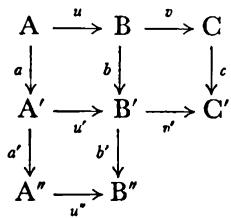
\includegraphics[keepaspectratio]{images/part001_696e1539.jpg}}

Suppose that: (1) \((u, v)\) and \((b, b')\) are exact sequences; (2) \(v' \circ u' = 0\) and \(a' \circ a = 0\) ; (3) \(c\) and \(u'\) are injective and \(a'\) is surjective. Show that under these conditions \(u''\) is injective.

\begin{enumerate}
\def\labelenumi{\arabic{enumi}.}
\setcounter{enumi}{2}
\tightlist
\item
  Consider a commutative diagram of commutative groups
\end{enumerate}

\pandocbounded{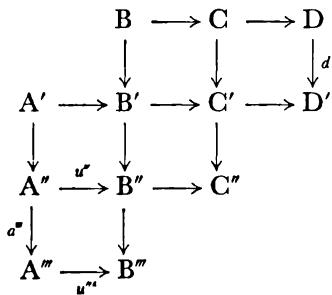
\includegraphics[keepaspectratio]{images/part001_1549be15.jpg}}

in which the rows and columns are assumed to be exact, d and \(u''\) injective and \(a''\) surjective. Show that under these conditions \(u'''\) is injective. Generalize this result.

\begin{enumerate}
\def\labelenumi{\arabic{enumi}.}
\setcounter{enumi}{3}
\tightlist
\item
  Consider a commutative diagram of commutative groups
\end{enumerate}

\pandocbounded{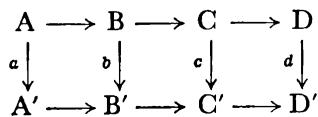
\includegraphics[keepaspectratio]{images/part001_0674edfc.jpg}}

where the two rows are assumed to be exact.

\begin{enumerate}
\def\labelenumi{(\alph{enumi})}
\item
  Show that, if \(a\) is surjective and \(b\) and \(d\) injective, then \(c\) is injective.
\item
  Show that, if \(d\) is injective and \(a\) and \(c\) surjective, then \(b\) is surjective.
\end{enumerate}

\begin{enumerate}
\def\labelenumi{\arabic{enumi}.}
\setcounter{enumi}{4}
\tightlist
\item
  Suppose that an exact sequence \(A^{\prime} \xrightarrow{u} A \xrightarrow{v} A^{\prime\prime} \to 0\) and two surjective homomorphisms \(B^{\prime} \xrightarrow{a^{\prime}} A^{\prime}, B^{\prime\prime} \xrightarrow{a^{\prime\prime}} A^{\prime\prime}\) are given, where A, A', A'', B', B'' are modules over the same ring. Show that, if \(B^{\prime\prime}\) is a projective module, there exists a surjective homomorphism \(a: B^{\prime} \oplus B^{\prime\prime} \to A\) such that the diagram
\end{enumerate}

\pandocbounded{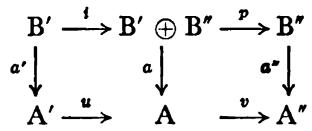
\includegraphics[keepaspectratio]{images/part001_093beead.jpg}}

is commutative (i and p being the canonical mappings).

\begin{enumerate}
\def\labelenumi{\arabic{enumi}.}
\setcounter{enumi}{5}
\tightlist
\item
  Suppose that an exact sequence \(0 \to A' \xrightarrow{u} A \xrightarrow{v} A''\) and two injective homomorphisms \(A' \xrightarrow{a'} C', A'' \xrightarrow{a''} C''\) are given, where \(A, A', A'', C', C''\) are modules over the same ring. Show that, if \(C'\) is an injective module (Algebra, Chapter II, § 2, Exercise 11), there exists an injective homomorphism \(a: A \to C' \oplus C''\) such that the diagram
\end{enumerate}

\pandocbounded{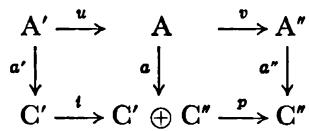
\includegraphics[keepaspectratio]{images/part001_5ee4bea9.jpg}}

are commutative (i and p being the canonical mappings).

\begin{enumerate}
\def\labelenumi{\arabic{enumi}.}
\setcounter{enumi}{6}
\tightlist
\item
  Let U, V, W be three commutative groups and \(f: \mathrm{U} \to \mathrm{V}\) , \(g: \mathrm{V} \to \mathrm{W}\) homomorphisms.
\end{enumerate}

\begin{enumerate}
\def\labelenumi{(\alph{enumi})}
\tightlist
\item
  Consider the diagram
\end{enumerate}

\pandocbounded{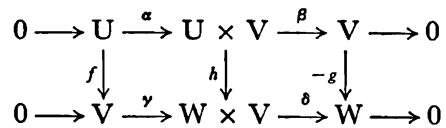
\includegraphics[keepaspectratio]{images/part001_5d67b0a0.jpg}}

where \(\alpha(u) = (u, f(u)), \beta(u, v) = v - f(u), \gamma(v) = (g(v), v), \delta(w, v) = w - g(v)\) , \(h(u, v) = (g(f(u)), v)\) . Show that this diagram is commutative and that its rows are exact.

\begin{enumerate}
\def\labelenumi{(\alph{enumi})}
\setcounter{enumi}{1}
\tightlist
\item
  Deduce from (a) and Proposition 2 of no. 4 an exact sequence
\end{enumerate}

\[
\begin{array}{c} 0 \to \operatorname{Ker} (f) \to \operatorname{Ker} (g \circ f) \to \operatorname{Ker} (g) \to \operatorname{Coker} (f) \to \operatorname{Coker} (g \circ f) \to \\ \operatorname{Coker} (g) \to 0. \end{array}
\]

Give a direct definition of this exact sequence.

\exercisesection{2}

\begin{enumerate}
\def\labelenumi{\arabic{enumi}.}
\item
  Give an example of an exact sequence \(0 \rightarrow N' \rightarrow N \rightarrow N'' \rightarrow 0\) of left A-modules and a right A-module E such that E is \(N'\) -flat and \(N''\) -flat, but not N-flat (take for example \(N' = N'' = Z/2Z\) ).
\item
  Let M, N be two submodules of an A-module E such that \(M + N\) is flat. For M and N to be flat, it is necessary and sufficient that \(M \cap N\) be flat.
\item
  Let A be the ring K{[}X, Y{]} of polynomials in two indeterminates over a field K.
\end{enumerate}

\begin{enumerate}
\def\labelenumi{(\alph{enumi})}
\item
  Consider in A the principal ideals \(\mathfrak{b} = (\mathbf{X}), \mathfrak{c} = (\mathbf{Y})\) , which are free A-modules and whose intersection \(\mathfrak{b} \cap \mathfrak{c} = (\mathbf{XY})\) is also free. Show that \(\mathfrak{a} = \mathfrak{b} + \mathfrak{c}\) is not a flat A-module, although \(\mathfrak{a}\) is torsion-free (cf.~Algebra, Chapter III, § 2, Exercise 4).
\item
  In the A-module \(A^{2}\) , let R be the submodule consisting of the elements \((x, -x)\) where \(x \in a\) . In the A-module \(A^{2}/R\) , let M, N be the submodules which are the images of the factor submodules of \(A^{2}\) ; show that M and N are isomorphic to A, but that \(M \cap N\) is not a flat A-module.
\end{enumerate}

\begin{enumerate}
\def\labelenumi{\arabic{enumi}.}
\setcounter{enumi}{3}
\tightlist
\item
  \begin{enumerate}
  \def\labelenumii{(\alph{enumii})}
  \tightlist
  \item
    Give an example of an exact sequence
  \end{enumerate}
\end{enumerate}

\[
0 \rightarrow \mathrm{E} ^ {\prime} \rightarrow \mathrm{E} \rightarrow \mathrm{E} ^ {\prime \prime} \rightarrow 0
\]

which does not split and all of whose terms are flat modules (cf.~Algebra, Chapter VII, § 3, Exercise 8 (b)).

\begin{enumerate}
\def\labelenumi{(\alph{enumi})}
\setcounter{enumi}{1}
\tightlist
\item
  From (a) deduce an example of an exact sequence
\end{enumerate}

\[
0 \rightarrow \mathrm{E} ^ {\prime} \rightarrow \mathrm{E} \rightarrow \mathrm{E} ^ {\prime \prime} \rightarrow 0
\]

which does not split and whose terms are right A-modules which are not flat, such that for every left A-module F the sequence

\[
0 \rightarrow \mathrm{E} ^ {\prime} \otimes \mathrm{F} \rightarrow \mathrm{E} \otimes \mathrm{F} \rightarrow \mathrm{E} ^ {\prime \prime} \otimes \mathrm{F} \rightarrow 0
\]

is exact (use Lemma 2 of no. 1).

\begin{enumerate}
\def\labelenumi{\arabic{enumi}.}
\setcounter{enumi}{4}
\tightlist
\item
  Give an example of a right A-module E, a left A-module F and two submodules \(F'\) , \(F''\) of F such that the canonical image of \(E \otimes (F' \cap F'')\) in \(E \otimes F\) is not the intersection of the canonical images of \(E \otimes F'\) and \(E \otimes F''\) (cf.~Exercise 3(a)).
\end{enumerate}

¶ 6. Let A be a ring and M a left A-module. An exact sequence

\[
\mathrm{L} _ {n} \rightarrow \mathrm{L} _ {n - 1} \rightarrow \dots \rightarrow \mathrm{L} _ {1} \rightarrow \mathrm{L} _ {0} \rightarrow \mathrm{M} \rightarrow 0
\]

where \(L_{i}\) is a free left A-module ( \(0 \leqslant i \leqslant n\) ), is called a presentation of M of length n or an n-presentation of M. The presentation is called finite if all the \(L_{i}\) are finitely generated free modules.

If M is a finitely generated left A-module, we denote by \(\lambda(M)\) the least upper bound (finite or \(+\infty\) ) of the integers \(n \geqslant 0\) such that M has a finite \(n\) -presentation. If M is not finitely generated, we set \(\lambda(M) = -1\) .

\begin{enumerate}
\def\labelenumi{(\alph{enumi})}
\item
  Let \(0 \to \mathbf{P} \to \mathbf{N} \to \mathbf{M} \to 0\) be an exact sequence of left A-modules. Then \(\lambda(\mathbf{N}) \geqslant \inf(\lambda(\mathbf{P}), \lambda(\mathbf{M}))\) . (Starting with two \(n\) -presentations of \(\mathbf{P}\) and \(\mathbf{M}\) respectively, derive one for \(\mathbf{N}\) using Exercise 5 of § 1.)
\item
  Let \(M_{n} \xrightarrow{u_{n}} M_{n-1} \rightarrow \cdots \rightarrow M_{0} \xrightarrow{u_{0}} M \rightarrow 0\) be a finite n-presentation of M; show that, if \(\lambda(M) > n\) , \(\operatorname{Ker}(u_{n})\) is a finitely generated A-module. (Let
\end{enumerate}

\[
\mathrm{L} _ {n + 1} \xrightarrow {v _ {n + 1}} \mathrm{L} _ {n} \longrightarrow \dots \longrightarrow \mathrm{L} _ {2} \xrightarrow {v _ {2}} \mathrm{L} _ {1} \xrightarrow {v _ {1}} \mathrm{L} _ {0} \xrightarrow {v _ {0}} \mathrm{M} \longrightarrow 0
\]

be a finite \((n + 1)\) -presentation of \(\mathbf{M}\) and let \(\mathbf{P} = \operatorname{Ker}(v_0)\) be such that there is an \(n\) -presentation of \(\mathbf{P}\) :

\[
\mathrm{L} _ {n + 1} \xrightarrow {v _ {n + 1}} \mathrm{L} _ {n} \longrightarrow \dots \longrightarrow \mathrm{L} _ {2} \xrightarrow {v _ {2}} \mathrm{L} _ {1} \xrightarrow {v _ {1}} \mathrm{P} \longrightarrow 0.
\]

Applying the method of (a) to the exact sequence \(0 \rightarrow P \rightarrow L_{0} \rightarrow M \rightarrow 0\) we obtain an exact sequence

\[
\mathrm{M} _ {n} \oplus \mathrm{L} _ {n + 1} \xrightarrow {w _ {n}} \mathrm{M} _ {n - 1} \oplus \mathrm{L} _ {n} \xrightarrow {w _ {n - 1}} \dots \xrightarrow {w _ {1}} \mathrm{M} _ {0} \oplus \mathrm{L} _ {1} \xrightarrow {w _ {0}} \mathrm{L} _ {0} \longrightarrow 0
\]

and exact sequences \(0 \to \operatorname{Ker}(v_{i+1}) \to \operatorname{Ker}(w_i) \to \operatorname{Ker}(u_i) \to 0\) (§ 1, no. 4, Proposition 2). Observe finally that \(\operatorname{Ker}(w_i)\) is a direct factor of \(\mathbf{M}_i \oplus \mathbf{L}_{i+1}\) .

\begin{enumerate}
\def\labelenumi{(\alph{enumi})}
\setcounter{enumi}{2}
\tightlist
\item
  Show that with the hypotheses of (a)
\end{enumerate}

\[
\lambda (\mathbf {M}) \geqslant \inf (\lambda (\mathbf {N}), \lambda (\mathbf {P}) + 1).
\]

(If \(n \leqslant \inf(\lambda(N), \lambda(P) + 1)\) , show by induction on \(n\) that \(\lambda(M) \geqslant n\) , arguing as in (a) and using (b).)

\begin{enumerate}
\def\labelenumi{(\alph{enumi})}
\setcounter{enumi}{3}
\tightlist
\item
  Show that with the hypotheses of (a)
\end{enumerate}

\[
\lambda (\mathrm{P}) \geqslant \inf (\lambda (\mathrm{N}), \lambda (\mathrm{M}) - 1).
\]

(Same method as in (c).) Deduce that, if \(\lambda(N) = +\infty\) , then \(\lambda(M) = \lambda(P) + 1\) .

\begin{enumerate}
\def\labelenumi{(\alph{enumi})}
\setcounter{enumi}{4}
\tightlist
\item
  Deduce from (a), (c) and (d) that, if \(\mathbf{N} = \mathbf{M} \oplus \mathbf{P}\) , then
\end{enumerate}

\[
\lambda (\mathbf {N}) = \inf (\lambda (\mathbf {M}), \lambda (\mathbf {P})).
\]

In particular, for N to admit a finite presentation it is necessary and sufficient that M and P do so too.

\begin{enumerate}
\def\labelenumi{(\alph{enumi})}
\setcounter{enumi}{5}
\tightlist
\item
  Let \(N_{1}\) , \(N_{2}\) be two submodules of an A-module M. Suppose that \(N_{1}\) and \(N_{2}\) admit finite presentations. For \(N_{1} + N_{2}\) to admit a finite presentation it is necessary and sufficient that \(N_{1} \cap N_{2}\) be finitely generated.
\end{enumerate}

\begin{enumerate}
\def\labelenumi{\arabic{enumi}.}
\setcounter{enumi}{6}
\tightlist
\item
  \begin{enumerate}
  \def\labelenumii{(\alph{enumii})}
  \tightlist
  \item
    With the notation of Exercise 6, show that, if M is a projective module, then \(\lambda(M) = -1\) or \(\lambda(M) = +\infty\) . If A is a left Noetherian ring, then, for every A-module M, \(\lambda(M) = -1\) or \(\lambda(M) = +\infty\) .
  \end{enumerate}
\end{enumerate}

\begin{enumerate}
\def\labelenumi{(\alph{enumi})}
\setcounter{enumi}{1}
\item
  If \(\mathfrak{a}\) is a left ideal of a ring \(\mathbf{A}\) , which is not finitely generated, \(\mathbf{A}_s / \mathfrak{a}\) is a monogenous A-module which does not admit a finite presentation, in other words \(\lambda(\mathbf{A}_s / \mathfrak{a}) = 0\) (no. 8, Lemma 9).
\item
  Give an example of a monogenous left ideal \(\mathfrak{a}\) of a ring A such that \(\mathbf{A}_s / \mathfrak{a}\) (which has a finite presentation) admits a dual which is not a finitely generated right A-module.
\item
  Let K be a commutative field, E the vector space \(\mathbf{K}^{(\mathbf{N})}, (e_n)\) the canonical basis of E and T the tensor algebra of E, which therefore has a basis consisting of the finite products \(e_{i_1}e_{i_2}\ldots e_{i_k}\) ( \(k \geqslant 0, i_j \in N\) for all j). For a given integer n, let b be the two-sided ideal of T generated by the products
\end{enumerate}

\[
e _ {1} e _ {0}, e _ {2} e _ {1}, \dots , e _ {n} e _ {n - 1}
\]

and \(e_{n+k}e_n\) for all \(k\geqslant 1\) ; let A be the quotient ring T/b, and for every integer \(m\) , let \(a_m\) be the canonical image of \(e_m\) in A. Show that, if \(\mathbf{M} = \mathbf{A}_s / \mathbf{A}a_0\) , then \(\lambda (\mathbf{M}) = n\) (observe that, for \(m\leqslant n - 1\) , the left annihilator of \(a_m\) is \(\mathrm{A}a_{m+1}\) and use Exercise 6(b)).

\begin{enumerate}
\def\labelenumi{\arabic{enumi}.}
\setcounter{enumi}{7}
\item
  Let C be a commutative ring and E, F two C-modules. Show that \(\lambda(E \otimes_{\mathbb{C}} F) \geqslant \inf(\lambda(E), \lambda(F))\) .
\item
  Let E be a finitely presented left A-module.
\end{enumerate}

\begin{enumerate}
\def\labelenumi{(\alph{enumi})}
\item
  Show that for every family \((\mathbf{F}_t)_{t \in I}\) of right A-modules, the canonical homomorphism \(\mathbf{E} \otimes_{\mathbf{A}} \left( \prod_{t \in I} \mathbf{F}_t \right) \to \prod_{t \in I} (\mathbf{E} \otimes_{\mathbf{A}} \mathbf{F}_t)\) (Algebra, Chapter II, § 3, no. 7) is bijective.
\item
  Let \((G_{\alpha}, \phi_{\beta\alpha})\) be a direct system of left A-modules; show that the canonical homomorphism
\end{enumerate}

\[
\varinjlim \operatorname{Hom} _ {\mathrm{A}} (\mathrm{E}, \mathrm{G} _ {\alpha}) \rightarrow \operatorname{Hom} _ {\mathrm{A}} (\mathrm{E}, \varinjlim \mathrm{G} _ {\alpha})
\]

is bijective.

\begin{enumerate}
\def\labelenumi{\arabic{enumi}.}
\setcounter{enumi}{9}
\tightlist
\item
  \begin{enumerate}
  \def\labelenumii{(\alph{enumii})}
  \tightlist
  \item
    Let A be a ring, I a set and R a submodule of \(L = A_{d}^{(I)}\) . Let S be the set of ordered pairs (J, S), where J is a finite subset of I and S a finitely generated submodule of \(A_{d}^{J} \cap R\) . S is ordered by the relation ``J ⊂ J' and S ⊂ S'\,''; show that S is directed with respect to this order relation, that the family ( \(A_{d}^{J}/S\) ) is a direct system of right A-modules with S as indexing set and that there exists an isomorphism of L/R onto \(\varinjlim (A_{d}^{J}/S)\) .
  \end{enumerate}
\end{enumerate}

\begin{enumerate}
\def\labelenumi{(\alph{enumi})}
\setcounter{enumi}{1}
\tightlist
\item
  Deduce from (a) that every A-module is a direct limit of finitely presented A-modules.
\end{enumerate}

\begin{enumerate}
\def\labelenumi{\arabic{enumi}.}
\setcounter{enumi}{10}
\tightlist
\item
  Let E be a right A-module. E is called pseudo-coherent if every finitely generated submodule of E is finitely presented; every submodule of a pseudo-coherent module is pseudo-coherent. E is called coherent if it is pseudo-coherent and finitely generated (and therefore finitely presented).
\end{enumerate}

\begin{enumerate}
\def\labelenumi{(\alph{enumi})}
\item
  Let \(0 \to E' \to E \to E'' \to 0\) be an exact sequence of right A-modules. Show that, if E is pseudo-coherent (resp. coherent) and \(E'\) is finitely generated \(E''\) is pseudo-coherent (resp. coherent). Show that, if \(E'\) and \(E''\) are pseudo-coherent (resp. coherent), so is E. Show that, if E and \(E''\) are coherent, so is \(E'\) (use Exercise 6 and Lemma 9 of no. 8).
\item
  Let E be a coherent A-module and \(E'\) a pseudo-coherent (resp. coherent) A-module. Show that, for every homomorphism \(u: E \to E'\) , \(\text{Im}(u)\) and \(\text{Ker}(u)\) are coherent and that \(\text{Coker}(u)\) is pseudo-coherent (resp. coherent) (use (a)).
\item
  Show that every direct sum (resp. every finite direct sum) of pseudo-coherent (resp. coherent) modules is a pseudo-coherent (resp. coherent) module.
\item
  If E is a pseudo-coherent module and M, N are coherent submodules of E, show that \(M + N\) and \(M \cap N\) are coherent (use (a) and (c)).
\item
  Suppose that A is commutative. Show that, if E is a coherent A-module and F a coherent (resp. pseudo-coherent) A-module, \(\operatorname{Hom}_{\mathbf{A}}(\mathbf{E}, \mathbf{F})\) is a coherent (resp. pseudo-coherent) A-module. (Reduce it to the case where F is coherent and consider a finite presentation of E, then use (b).)
\end{enumerate}

¶ 12. (a) Let A be a ring. Show that the following four properties are equivalent:

\((\alpha)\) The right A-module \(\mathbf{A}_d\) is coherent (Exercise 11).

(β) Every finitely presented right A-module is coherent.

(γ) Every A-module \(A_{s}^{I}\) (I an arbitrary set) is flat.

(δ) Every product of flat left A-modules is flat.

(To prove that \((\alpha)\) implies \((\beta)\) , use Exercise 11(b). To see that \((\gamma)\) implies \((\alpha)\) , use Proposition 13 of no. 11 and argue by reductio ad absurdum. To show that \((\alpha)\) implies \((\delta)\) , use Exercises 9.)

Such a ring is called right coherent and the concept of a left coherent ring is defined similarly.

\begin{enumerate}
\def\labelenumi{(\alph{enumi})}
\setcounter{enumi}{1}
\tightlist
\item
  Show that every right Noetherian ring is right coherent. Give an example of a right Artinian ring which is not left coherent (cf.~Algebra, Chapter VIII, § 2, Exercise 4).
\end{enumerate}

*(c) The ring of a non-discrete valuation of height 1 (Chapter VI) is coherent but contains ideals which are not coherent and admits (monogenous) quotient modules which are not pseudo-coherent.*

\begin{enumerate}
\def\labelenumi{(\alph{enumi})}
\setcounter{enumi}{3}
\item
  Show that, if A is a right coherent ring, then, for every right A-module E, \(\lambda(\mathrm{E}) = -1\) or \(\lambda(\mathrm{E}) = 0\) or \(\lambda(\mathrm{E}) = +\infty\) (Exercise 6).
\item
  Let \((\mathbf{A}_{\alpha}, \phi_{\beta \alpha})\) be a direct system of rings whose indexing set is directed and let \(\mathbf{A} = \varinjlim \mathbf{A}_{\alpha}\) . Suppose that, for \(\alpha \leqslant \beta\) , \(\mathbf{A}_{\beta}\) is a flat right \(\mathbf{A}_{\alpha}\) -module. Show that, if the \(\mathbf{A}_{\alpha}\) are right coherent, so is \(\mathbf{A}\) . (Observe that \(\mathbf{A}\) is a flat \(\mathbf{A}_{\alpha}\) -module for all \(\alpha\) and that, if \(\mathbf{E}\) is a finitely generated submodule of \(\mathbf{A}_d\) , there exists an index \(\alpha\) and a finitely generated submodule \(\mathbf{E}_{\alpha}\) of \((\mathbf{A}_{\alpha})_d\) such that \(\mathbf{E}_{\alpha} \otimes_{\mathbf{A}_{\alpha}} \mathbf{A}\) is isomorphic to \(\mathbf{E}\) .)
\end{enumerate}

* (f) Deduce from (e) that every polynomial ring (in any finite or infinite set of indeterminates) over a Noetherian commutative ring is coherent. Deduce from this that a quotient ring of a coherent ring is not necessarily coherent.*

\begin{enumerate}
\def\labelenumi{(\alph{enumi})}
\setcounter{enumi}{6}
\tightlist
\item
  For A to be left coherent, it is necessary and sufficient that the left annihilator of every element of A be finitely generated and that the intersection of two finitely generated left ideals of A be finitely generated (use Exercise 6(f)).
\end{enumerate}

¶ 13. Let A, B be two rings, F an (A, B)-bimodule and G a right B-module. Show that, if G is injective (Algebra Chapter II, § 2, Exercise 11) and F is a flat left A-module, the right A-module \(\operatorname{Hom}_{B}(F, G)\) is injective. (Use the isomorphism

\[
\operatorname{Hom} _ {\mathbf {A}} (\mathbf {E}, \operatorname{Hom} _ {\mathbf {B}} (\mathbf {F}, \mathbf {G})) \rightarrow \operatorname{Hom} _ {\mathbf {B}} (\mathbf {E} \otimes_ {\mathbf {A}} \mathbf {F}, \mathbf {G})
\]

for a right A-module E (Algebra, Chapter II, § 4, no. 1).)

¶ 14. Let A, B be two rings, E a left A-module, F an (A, B)-bimodule and G a right B-module; consider the canonical homomorphism (Algebra, Chapter II, § 4, Exercise 5)

\[
\sigma \colon \operatorname{Hom} _ {\mathbb {B}} (\mathrm{F}, \mathrm{G}) \otimes_ {\mathrm{A}} \mathrm{E} \rightarrow \operatorname{Hom} _ {\mathbb {B}} (\operatorname{Hom} _ {\mathrm{A}} (\mathrm{E}, \mathrm{F}), \mathrm{G})
\]

such that \((\sigma(u \otimes x))(v) = u(v(x))\) for all \(x \in \mathbf{E}\) , \(u \in \operatorname{Hom}_{\mathbf{B}}(\mathbf{F}, \mathbf{G})\) ,

\[
v \in \operatorname{Hom} _ {\mathbf {A}} (\mathrm{E}, \mathbf {F}).
\]

Show that, if G is an injective B-module (Algebra, Chapter II, § 2, Exercise 11) and E finitely presented, \(\sigma\) is bijective. (Consider first the case where E is free and finitely generated.)

¶ 15. Let A be a ring. Show that every left A-module E which is flat and finitely presented is projective. (Given a surjective left A-module homomorphism \(u: \mathbf{F} \to \mathbf{F}'\) , let \(u'\) be the homomorphism

\[
\operatorname{Hom} \left(1 _ {\mathbf {E}}, u\right): \operatorname{Hom} _ {\mathbf {A}} (\mathrm{E}, \mathrm{F}) \rightarrow \operatorname{Hom} _ {\mathbf {A}} (\mathrm{E}, \mathrm{F} ^ {\prime \prime})
\]

and \(\bar{u}\) the homomorphism

\[
\operatorname{Hom} \left(u ^ {\prime}, 1 _ {G}\right): \operatorname{Hom} _ {\mathbf {Z}} \left(\operatorname{Hom} _ {A} (E, F ^ {\prime \prime}), G\right)\rightarrow \operatorname{Hom} _ {\mathbf {Z}} \left(\operatorname{Hom} _ {A} (E, F), G\right),
\]

where G is a divisible Z-module. Using Exercise 14 first, prove that \(\bar{u}\) is injective; then, with a suitable choice for G (Algebra, Chapter II, §2, Exercise 14), show that \(u'\) is surjective.)

\begin{enumerate}
\def\labelenumi{\arabic{enumi}.}
\setcounter{enumi}{15}
\tightlist
\item
  Let A be a ring and \(a\) an element of A. Show that the following properties are equivalent.
\end{enumerate}

\((\alpha)\) \(a \in aAa\) .

(β) aA is a direct factor of the module \(A_{d}\) .

(γ) \(A_{d}/aA\) is a flat right A-module.

(δ) For every left ideal b of A, \(aA \cap b = ab\) .

(Use the Corollary to Proposition 7 of no. 6 to prove the equivalence of \((\gamma)\) and \((\delta)\) and show directly that \((\delta)\) implies \((\alpha)\) and \((\alpha)\) implies \((\beta)\) , by proving the existence of an idempotent element \(e \in a\mathbf{A}\) such that \(e\mathbf{A} = a\mathbf{A}\) .)

\begin{enumerate}
\def\labelenumi{\arabic{enumi}.}
\setcounter{enumi}{16}
\tightlist
\item
  Let A be a ring. Show that the following properties are equivalent:
\end{enumerate}

(α) Every element \(a \in A\) satisfies the equivalent properties of Exercise 16.

(β) Every finitely generated right ideal of A is a direct factor of \(A_{d}\) .

(γ) Every left A-module is flat.

(δ) Every right A-module is flat.

Then A is called an absolutely flat ring (*).

(To see that \((\alpha)\) implies \((\beta)\) , use Exercise 15(b) of Algebra, Chapter VIII, §6.)

¶ 18. Let A be an absolutely flat ring (Exercise 17).

\begin{enumerate}
\def\labelenumi{(\alph{enumi})}
\item
  Let P be a projective right A-module. Show that every finitely generated submodule E of P is a direct factor of P. (Reduce it to the case where P is free and finitely generated. Then note that P/E is finitely presented and use Exercises 15.)
\item
  Show that every projective right A-module P is the direct sum of monogenous submodules isomorphic to monogenous right ideals of A. (Use Kaplansky's Theorem (Algebra, Chapter II, § 2, Exercises 3) to reduce the problem to the case where P is generated by a countable family of elements, then use (a).)
\item
  Give an example of an absolutely flat ring A and a non-projective finitely generated A-module (consider a quotient of A by an ideal which is not finitely generated; cf.~Algebra, Chapter VIII, § 6, Exercise 15(f) and Commutative Algebra, Chapter II, § 4, Exercise 17).
\end{enumerate}

\begin{enumerate}
\def\labelenumi{\arabic{enumi}.}
\setcounter{enumi}{18}
\tightlist
\item
  Let A be a ring. Show that the following properties are equivalent:
\end{enumerate}

\((\alpha)\) A is semisimple.

(β) Every right ideal of A is an injective A-module.

(γ) Every right A-module is projective.

(δ) Every right A-module is injective.

\begin{enumerate}
\def\labelenumi{\arabic{enumi}.}
\setcounter{enumi}{19}
\item
  Let A be an integral domain, B an A-algebra which is a flat A-module and M a torsion-free A-module. Show that, if \(t \in B\) is not a divisor of zero, the relation t. z = 0 for \(z \in B \otimes_{A} M\) implies z = 0. (Reduce this to the case where M is finitely generated and, by embedding M in a finitely generated free A-module, to the case where M = A.)
\item
  Let S be a commutative ring, R a commutative S-algebra, B an S-algebra (commutative or otherwise) and \(\mathrm{B}_{(\mathrm{R})}\) the R-algebra obtained from B by extension of scalars. Suppose that R is a flat S-module and that B is a finitely generated S-module. If Z is the centre of B, show that the canonical homomorphism of \(Z_{(R)} = Z \otimes_{S} R\) to \(\mathrm{B}_{(\mathrm{R})}\) is an isomorphism of \(Z_{(R)}\) onto the centre of \(\mathrm{B}_{(\mathrm{R})}\) . (Use the exact sequence
\end{enumerate}

\[
0 \longrightarrow \mathrm{Z} \longrightarrow \mathrm{B} \stackrel {\theta} {\longrightarrow} \operatorname{Hom} _ {\mathrm{s}} (\mathrm{B}, \mathrm{B})
\]

where \(\theta (x)(y) = xy - yx\) , and Proposition 11 of no. 10.)

\begin{enumerate}
\def\labelenumi{\arabic{enumi}.}
\setcounter{enumi}{21}
\tightlist
\item
  Let E be a left A-module. For every right ideal a of A and every element \(a \in A\) , denote by a: a the set of \(x \in A\) such that \(ax \in a\) and by aE: a the set of \(y \in E\) such that \(ay \in aE\) . Then clearly (a: a)E ⊂ aE: a. Show that, for E to be flat, it is necessary and sufficient that, for every right ideal a of A and every element \(a \in A\) , (a: a)E = aE: a. (To see that the condition is necessary, consider the exact sequence of right A-modules \(0 \to (a: a)/a \stackrel{\psi}{\to} A_d/a \stackrel{\varphi}{\to} A_d/a\) , where \(\psi\) is the canonical injection and \(\phi\) the mapping obtained by taking quotients under left multiplication by a. To see that the condition is sufficient apply the criterion of Corollary 1 to Proposition 13 of no. 11: starting with a relation \(\sum_{i=1}^{n} a_i x_i = 0\) , where \(a_i \in A\) , \(x_i \in E\) , apply the hypothesis to the ideal
\end{enumerate}

\(a_{2}=\sum_{i=2}^{n}a_{i}A\) and the element \(a_{1}\) and argue by induction on n.)

\begin{enumerate}
\def\labelenumi{\arabic{enumi}.}
\setcounter{enumi}{22}
\tightlist
\item
  \begin{enumerate}
  \def\labelenumii{(\alph{enumii})}
  \tightlist
  \item
    Let \(0 \to \mathbf{R} \to \mathbf{L} \to \mathbf{E} \to 0\) be an exact sequence of left A-modules, where \(\mathbf{L}\) is a free A-module; let \((e_{\alpha})\) be a basis of \(\mathbf{L}\) . Show that the following conditions are equivalent:
  \end{enumerate}
\end{enumerate}

(α) E is flat.

(β) For all \(x \in \mathbb{R}\) , if \(\mathfrak{a}_x\) is the right ideal generated by the components of \(x\) with respect to the basis \((e_{\alpha})\) , then \(x \in \mathbb{R}\mathfrak{a}_x\) .

\((\gamma)\) For all \(x \in \mathbb{R}\) , there exists a homomorphism \(u_x: \mathbf{L} \to \mathbf{R}\) such that \(u_x(x) = x\) .

\begin{enumerate}
\def\labelenumi{(\arabic{enumi})}
\setcounter{enumi}{7}
\tightlist
\item
  For every finite sequence \((x_{i})_{1\leqslant i\leqslant n}\) of elements of R, there exists a homomorphism \(u\colon \mathbf{L}\to \mathbb{R}\) such that \(u(x_{i}) = x_{i}\) for \(1\leqslant i\leqslant n\) . (Use the Corollary to Proposition 7 of no. 6.)
\end{enumerate}

\begin{enumerate}
\def\labelenumi{(\alph{enumi})}
\setcounter{enumi}{1}
\tightlist
\item
  Let \(\mathfrak{a}\) be a left ideal of \(\mathbf{A}\) such that \(\mathbf{A} / \mathfrak{a}\) is a flat \(\mathbf{A}\) -module. Show that, for every finitely generated left ideal \(\mathfrak{b} \subset \mathfrak{a}\) , there exists \(x \in \mathbf{A}\) such that
\end{enumerate}

\[
\mathfrak {b} \subset \mathrm{A} x \subset \mathfrak {a}
\]

(use condition (δ) of (a)).

\begin{enumerate}
\def\labelenumi{(\alph{enumi})}
\setcounter{enumi}{2}
\item
  Derive from (a) a new proof of the result of Exercise 15.
\item
  Let \(\mathfrak{r}\) be the Jacobson radical of \(\mathbf{A}\) and \(0 \to \mathbf{R} \to \mathbf{L} \to \mathbf{E} \to 0\) an exact sequence of left A-modules such that \(\mathbf{L}\) is free. Suppose that \(\mathbf{E}\) is flat and \(\mathbf{R}\) is contained in \(\mathfrak{rL}\) . Show that \(\mathbf{R} = 0\) (in the notation of (a) observe that \(\mathfrak{a}_x\) is a finitely generated ideal and that \(\mathfrak{a}_x = \mathfrak{a}_x\mathfrak{r}\) ).
\item
  Let E be a finitely generated flat A-module; suppose that there exists a two-sided ideal b of A contained in the Jacobson radical of A such that E/bE is a free (A/b)-module. Show that E is then a free A-module (observe that there exists a finitely generated free A-module L such that L/bL is isomorphic to E/bE and use Algebra, Chapter VIII, § 6, no. 3, Corollary 4 to Proposition 6; then apply (d)).
\end{enumerate}

\begin{enumerate}
\def\labelenumi{\arabic{enumi}.}
\setcounter{enumi}{23}
\tightlist
\item
  A submodule \(M'\) of a right A-module M is called pure if, denoting by \(j: M' \rightarrow M\) the canonical injection, the homomorphism
\end{enumerate}

\[
j \otimes 1 _ {N} \colon M ^ {\prime} \otimes_ {A} N \rightarrow M \otimes_ {A} N
\]

is injective for every left A-module N. This is so if \(M'\) is a direct factor of M or if \(M/M'\) is flat, but these two conditions are not necessary (Exercise 4).

\begin{enumerate}
\def\labelenumi{(\alph{enumi})}
\item
  Show that, for \(\mathbf{M}'\) to be a pure submodule of \(\mathbf{M}\) , it is necessary and sufficient that, if \((m_i')_{i\in I}\) is a finite family of elements of \(\mathbf{M}'\) , \((x_j)_{j\in J}\) a family of elements of \(\mathbf{M}\) such that \(m_i' = \sum_{j\in J} x_j a_{jl}\) for all \(i\in I\) and a family \((a_{jl})\) of elements of \(\mathbf{A}\) , then there exists a family \((x_j')_{j\in J}\) of elements of \(\mathbf{M}'\) such that \(m_i' = \sum_{j\in J} x_j' a_{jl}\) for all \(i\in I\) . (To see that the condition is sufficient, use Lemma 10 of no. 11 to show that \(\mathbf{M}' \otimes_{\mathbf{A}} \mathbf{N} \to \mathbf{M} \otimes_{\mathbf{A}} \mathbf{N}\) is injective for every finitely generated left A-module \(\mathbf{N}\) ; to see that the condition is necessary, consider a finitely generated left A-module \(\mathbf{N} = \mathbf{L}/\mathbf{R}\) , where \(\mathbf{L}\) is a finitely generated free A-module and \(\mathbf{R}\) is a finitely generated submodule of \(\mathbf{L}\) .) Deduce from this criterion that, if \(\mathbf{A}\) is a principal ideal domain, the notion of pure submodule of an A-module coincides with that of Algebra, Chapter VII, § 2, Exercise 7.
\item
  Let M be a right A-module, M' a submodule of M and M'' a submodule of M'. Show that, if M' is a pure submodule of M and M'' a pure submodule of M', then M'' is a pure submodule of M and M'/M'' is a pure submodule of M/M''. If M'' is a pure submodule of M, M'' is a pure submodule of M'.
\item
  Show that, if N and P are two submodules of M such that \(N \cap P\) and \(N + P\) are pure in M, then N and P are pure submodules of M. Give an example of two submodules N, P of \(Z^{2}\) which are pure in \(Z^{2}\) but where \(N + P\) is not a pure submodule of \(Z^{2}\) .
\item
  Let C be a commutative ring and E, F two C-modules; show that, if \(E'\) (resp. \(F'\) ) is a pure submodule of E (resp. F), the canonical mapping \(E' \otimes_{C} F' \to E \otimes_{C} F\) is injective and identifies \(E' \otimes_{C} F'\) with a pure submodule of \(E \otimes_{C} F\) .
\item
  Let \(\rho: \mathbf{A} \to \mathbf{B}\) be a ring homomorphism, \(\mathbf{M}\) a right A-module and \(\mathbf{M}'\) a pure submodule of \(\mathbf{M}\) . Show that \(\mathbf{M}_{(\mathbf{B})}' = \mathbf{M}' \otimes_{\mathbf{A}} \mathbf{B}\) is canonically identified with a pure submodule of \(\mathbf{M}_{(\mathbf{B})} = \mathbf{M} \otimes_{\mathbf{A}} \mathbf{B}\) .
\end{enumerate}

\exercisesection{3}

\begin{enumerate}
\def\labelenumi{\arabic{enumi}.}
\tightlist
\item
  \begin{enumerate}
  \def\labelenumii{(\alph{enumii})}
  \tightlist
  \item
    For the direct sum of a family \((\mathbf{E}_{\lambda})\) of A-modules to be faithfully flat, it is sufficient that each of the \(E_{\lambda}\) be flat and that at least one of them be faithfully flat.
  \end{enumerate}
\end{enumerate}

\begin{enumerate}
\def\labelenumi{(\alph{enumi})}
\setcounter{enumi}{1}
\tightlist
\item
  Deduce from (a) that, if A is a simple ring, every non-empty A-module is faithfully flat. Is the result true for semisimple rings?
\end{enumerate}

\begin{enumerate}
\def\labelenumi{\arabic{enumi}.}
\setcounter{enumi}{1}
\item
  Let \((p_n)\) be the strictly increasing sequence of prime numbers and A the product ring \(\prod_{n} \mathbf{Z} / p_n \mathbf{Z}\) . Show that the direct sum E of the \(\mathbf{Z} / p_n \mathbf{Z}\) is a faithful projective A-module which is not faithfully flat (observe that E is an ideal of A such that \(\mathrm{E}^2 = \mathrm{E}\) ).
\item
  Let A be a right coherent ring (§ 2, Exercise 12). For a product of left A-modules to be faithfully flat, it is sufficient that each of them be flat and that at least one of them be faithfully flat.
\end{enumerate}

Deduce that, if A is a coherent commutative ring, the ring of formal power series \(A[[X_{1},\ldots,X_{n}]]\) is a faithfully flat A-module.

\begin{enumerate}
\def\labelenumi{\arabic{enumi}.}
\setcounter{enumi}{3}
\item
  Let A be a simple algebra over a commutative field K and B a subalgebra of A which is semisimple but not simple. Show that A is a faithfully flat (right or left) B-module, but that there exist right B-modules E which are not faithfully flat, whilst \(E \otimes_{B} A\) is always faithfully flat (Exercise 1).
\item
  Let A be a commutative ring and M a flat A-module containing a submodule N which is not a flat module (cf.~§ 2, Exercise 3). Let B (resp. C) be the A-module A ⊕ N (resp. A ⊕ M) in which multiplication is defined by \((a, x)(a', x') = (aa', ax' + a'x)\) ; then B is not a flat A-module, but the B-module C is a faithfully flat A-module and consequently B satisfies the conditions of Proposition 8 of no. 5.
\item
  Give an example of an integral domain A and a ring B of which A is a subring, such that B is a flat A-module but there exists an A-module E which is neither projective nor finitely generated, for which \(B \otimes_{A} E\) is a finitely generated free B-module.
\item
  If K is a field, the ring K{[}X{]} and the field K(X) are faithfully flat K-modules, but K(X) is not a faithfully flat K{[}X{]}-module.
\item
  Let \(p\) be a prime number and \(\mathbf{A}\) the subring of \(\mathbf{Q}\) consisting of the fractions \(k / p^n\) , where \(k \in \mathbf{Z}\) , \(n \geqslant 0\) . Show that \(\mathbf{A}\) is a flat \(\mathbf{Z}\) -module and that there exists a \(\mathbf{Z}\) -module \(\mathbf{E}\) which is not flat but where \(\mathbf{A} \otimes_{\mathbf{Z}} \mathbf{E}\) is a flat \(\mathbf{A}\) -module.
\item
  Let A be a commutative ring, B an A-algebra, \((\mathbf{C}_{\lambda})_{\lambda \in L}\) , a family of A-algebras and \(B_{\lambda} = C_{\lambda} \otimes_{A} B\) the tensor product algebra of \(C_{\lambda}\) and B for all \(\lambda \in L\) . Let E be a left B-module. Set \(E_{\lambda} = B_{\lambda} \otimes_{B} E = C_{\lambda} \otimes_{A} E\) ; this is a \((\mathbf{B}_{\lambda}, \mathbf{C}_{\lambda})\) -bimodule. Similarly, if F is a right B-module, set
\end{enumerate}

\[
\mathbf {F} _ {\lambda} = \mathbf {F} \otimes_ {\mathbf {B}} \mathbf {B} _ {\lambda} = \mathbf {F} \otimes_ {\mathbf {A}} \mathbf {C} _ {\lambda},
\]

which is a \((\mathbf{C}_{\lambda},\mathbf{B}_{\lambda})\) -bimodule.

\begin{enumerate}
\def\labelenumi{(\alph{enumi})}
\item
  Show that the \((\mathbf{C}_{\lambda},\mathbf{C}_{\lambda})\) -bimodule \(\mathbf{F}_{\lambda}\otimes_{\mathbf{B}_{\lambda}}\mathbf{E}_{\lambda}\) is isomorphic to \((\mathbf{F}\otimes_{\mathbf{B}}\mathbf{E})\otimes_{\mathbf{A}}\mathbf{C}_{\lambda}\) .
\item
  Show that, if E is a flat (resp. faithfully flat) B-module, each of the \(E_{\lambda}\) is a flat (resp. faithfully flat) \(B_{\lambda}\) -module. The converse is true if we assume further that \(\bigoplus C_{\lambda}\) is a faithfully flat A-module.
\item
  Show that, if \(L\) is finite, each of the \(E_{\lambda}\) is a finitely generated projective \(B_{\lambda}\) -module and \(\bigoplus_{\lambda \in L} C_{\lambda}\) is a faithfully flat A-module, then \(E\) is a finitely generated projective B-module (use Proposition 12 of no. 6).
\end{enumerate}

\begin{enumerate}
\def\labelenumi{\arabic{enumi}.}
\setcounter{enumi}{9}
\tightlist
\item
  \begin{enumerate}
  \def\labelenumii{(\alph{enumii})}
  \tightlist
  \item
    Let \(\rho: A \to B\) be a ring homomorphism. Show that, for every left ideal \(a\) of \(A\) which is a left annihilator of a subset \(M\) of \(A\) , \(\rho^{-1}(Ba) = a\) .
  \end{enumerate}
\end{enumerate}

\begin{enumerate}
\def\labelenumi{(\alph{enumi})}
\setcounter{enumi}{1}
\tightlist
\item
  Deduce from (a) an example of a homomorphism \(\rho: A \to B\) such that right A-module \(B\) is not flat but \(\bar{\rho}^{-1}(Ba) = a\) holds for every left ideal \(a\) of \(A\) (cf.~§ 2, Exercise 17 and Algebra, Chapter VIII, § 3, Exercise 11 and § 2, Exercise 6 and Chapter IX, § 2, Exercise 4).
\end{enumerate}

\exercisesection{4}

\begin{enumerate}
\def\labelenumi{\arabic{enumi}.}
\tightlist
\item
  Show that in the statement of Proposition 2, condition (a) can be replaced by:
\end{enumerate}

\((a^{\prime})\operatorname{Tor}_{1}^{\mathbb{R}}(\rho_{*}(\mathbf{E}),\mathbf{F}) = 0\) for every monogenous right S-module E.

(To prove that (a') implies (a), consider first the case when E is generated by n elements and argue by induction on n.)

CHAPTER II(*)

\chapter{Localization}

The conventions of Chapter I remain in force in this chapter. Also, unless otherwise stated, all rings are assumed to be commutative.

Let A, B be two rings, \(\rho\) a homomorphism from A to B and M a B-module. When we speak of M as an A-module, we mean, unless otherwise stated, with the A-module structure \(\rho_{*}(\mathbf{M})\) (defined by the external law \((a,m)\mapsto\rho(a)m\) ).

\section{PRIME IDEALS}

\subsection{Definition of prime ideals}

DEFINITION 1. An ideal p of a ring A is called prime if the ring A/p is an integral domain.

By this definition, an ideal p of a ring A is prime if the following two conditions hold:

\begin{enumerate}
\def\labelenumi{(\arabic{enumi})}
\item
  \(\mathfrak{p} \neq \mathbf{A}\) ;
\item
  if \(x, y\) are two elements of \(A\) such that \(x \notin p\) and \(y \notin p\) , then \(xy \notin p\) .
\end{enumerate}

These conditions can also be expressed by saying that the product of any finite family of elements of \(\mathbb{C}\mathfrak{p}\) belongs to \(\mathbb{C}\mathfrak{p}\) , as applying this condition to the empty set yields \(1\notin\mathfrak{p}\) .

A maximal ideal m of A is prime since A/m is a field; then it follows from Krull's theorem (Algebra, Chapter I, § 8, no. 7, Theorem 2) that every ideal of

A other than A is contained in at least one prime ideal. In particular, for prime ideals to exist in a ring A, it is necessary and sufficient that A be not reduced to 0.

Let \(f: \mathbf{A} \to \mathbf{B}\) be a ring homomorphism and \(q\) an ideal of \(\mathbf{B}\) . Set \(p = \bar{f}^{-1}(q)\) ; the homomorphism \(\overline{f}: \mathbf{A}/p \to \mathbf{B}/q\) derived from \(f\) by taking quotients is injective. Suppose that \(q\) is prime; as the ring \(B/q\) is an integral domain, so is \(A/p\) , being isomorphic to a subring of \(B/q\) ; consequently the ideal \(p = \bar{f}^{-1}(q)\) is prime. In particular, let \(A\) be a subring of \(B\) ; for every ideal \(q\) of \(B, q \cap A\) is a prime ideal \(A\) . If \(f\) is surjective, \(\overline{f}\) is an isomorphism; the conditions `` \(p\) is prime'' and `` \(q\) is prime'' are then equivalent. Hence, if \(p\) and \(a\) are ideals of \(A\) such that \(a \subset p\) , a necessary and sufficient condition for \(p\) to be prime is that \(p/a\) be prime in \(A/a\) .

PROPOSITION 1. Let A be a ring, \(\mathfrak{a}_1, \mathfrak{a}_2, \ldots, \mathfrak{a}_n\) ideals of A and p a prime ideal of A. If p contains the product \(\mathfrak{a}_1\mathfrak{a}_2 \ldots \mathfrak{a}_n\) , it contains at least one of the \(\mathfrak{a}_t\) .

Suppose in fact that \(\mathfrak{p}\) contains none of the \(a_{i}\) . For \(1 \leqslant i \leqslant n\) there exists then an element \(s_{i} \in a_{i} \cap \mathbb{C}p\) ; then \(s = s_{1}s_{2} \ldots s_{n}\) is contained in \(a_{1}a_{2} \ldots a_{n}\) and is not contained in \(\mathfrak{p}\) , which is absurd.

COROLLARY. Let \(\mathfrak{m}\) be a maximal ideal of \(\mathbf{A}\) ; for every integer \(n > 0\) , the only prime ideal containing \(\mathfrak{m}^n\) is \(\mathfrak{m}\) .

Such an ideal \(\mathfrak{p}\) must contain \(\mathfrak{m}\) by Proposition 1 applied to \(a_{i} = \mathfrak{m}\) for \(1 \leqslant i \leqslant n\) ; as \(\mathfrak{m}\) is maximal, \(\mathfrak{p} = \mathfrak{m}\) .

PROPOSITION 2. Let A be a ring, a a non-empty set of A which is closed under addition and multiplication and \((\mathfrak{p}_{i})_{i\in I}\) a non-empty finite family of ideals of A. Suppose that a is contained in the union of the \(p_{i}\) and that at most two of the \(p_{i}\) are not prime. Then a is contained in one of the \(p_{i}\) .

We argue by induction on \(n = \operatorname{Card}(\mathbf{I})\) ; the proposition is trivial if \(n = 1\) . Suppose that \(n \geqslant 2\) ; if there exists an index \(j\) such that \(\mathfrak{a} \cap \mathfrak{p}_j \subset \bigcup_{i \neq j} \mathfrak{p}_i\) , the set \(\mathfrak{a}\) , which is the union of the \(\mathfrak{a} \cap \mathfrak{p}_i\) where \(i \in \mathbf{I}\) , is contained in \(\bigcup_{i \neq j} \mathfrak{p}_i\) and hence in one of the \(\mathfrak{p}_i\) by the induction hypothesis. Suppose then that such an index does not exist; for every \(j \in \mathbf{I}\) let \(y_j\) be an element of \(\mathfrak{a} \cap \mathfrak{p}_j\) not belonging to any \(\mathfrak{p}_i\) for \(i \neq j\) . Let \(k\) be an element of \(\mathbf{I}\) chosen in such a way that \(\mathfrak{p}_k\) is prime if \(n > 2\) and chosen arbitrarily if \(n = 2\) ; let \(z = y_k + \prod_{i \neq k} y_i\) . Then \(z \in \mathfrak{a}\) , since \(\mathfrak{a}\) is closed under addition and multiplication; if \(j \neq k, \prod_{i \neq k} y_i\) belongs to \(\mathfrak{p}_j\) , but \(y_k \notin \mathfrak{p}_j\) , whence \(z \notin \mathfrak{p}_j\) . On the other hand, \(\prod_{i \neq k} y_i\) does not belong to \(\mathfrak{p}_k\) , as none of the factors \(y_i (i \neq k)\) belongs to it and \(\mathfrak{p}_k\) is prime if \(n - 1 > 1\) ; as \(y_k \in \mathfrak{p}_k\) , \(z\) does not belong to \(\mathfrak{p}_k\) and the proposition is established.

\subsection{Relatively prime ideals}

Let A be a ring; two ideals a, b of A are called relatively prime if \(a + b = A\) . For this to be true, it is necessary and sufficient that \(a + b\) be contained in no prime ideal (Algebra, Chapter I, § 8, no. 7, Theorem 2), in other words, that no prime ideal contain both a and b. Two distinct maximal ideals are relatively prime.

If A is a principal ideal domain (Algebra, Chapter VII, § 1), for two elements \(a\) , \(b\) of A to be relatively prime, it is necessary and sufficient, by Bezout's identity (loc. cit., no. 2, Theorem 1), that the ideals \(Aa\) and \(Ab\) be relatively prime.

PROPOSITION 3. Let a and b be two relatively prime ideals of a ring A. Let a' and b' be two ideals of A such that every element of a (resp. b) has a power in a' (resp. b'). Then a' and b' are relatively prime.

Under the given hypothesis, every prime ideal which contains \(a'\) contains a and every prime ideal which contains \(b'\) contains b. If a prime ideal contains \(a'\) and \(b'\) , then it contains a and b, which is absurd, since a and b are relatively prime; hence \(a'\) and \(b'\) are relatively prime.

PROPOSITION 4. Let \(\mathfrak{a}, \mathfrak{b}_1, \ldots, \mathfrak{b}_n\) be ideals of a ring \(\mathbf{A}\) . If \(\mathfrak{a}\) is relatively prime to each of the \(\mathfrak{b}_i (1 \leqslant i \leqslant n)\) , it is relatively prime to \(\mathfrak{b}_1\mathfrak{b}_2 \ldots \mathfrak{b}_n\) .

Let \(\mathfrak{p}\) be a prime ideal of \(\mathbf{A}\) . If \(\mathfrak{p}\) contains \(\mathfrak{a}\) and \(\mathfrak{b}_1\mathfrak{b}_2\ldots \mathfrak{b}_n\) , it contains one of the \(\mathfrak{b}_i\) (no. 1, Proposition 1), which is absurd since \(\mathfrak{a}\) and \(\mathfrak{b}_i\) are relatively prime.

PROPOSITION 5. Let \((a_{i})_{i\in I}\) be a non-empty finite family of ideals of a ring A. The following properties are equivalent:

\begin{enumerate}
\def\labelenumi{(\alph{enumi})}
\item
  For \(i \neq j\) , \(\mathfrak{a}_i\) and \(\mathfrak{a}_j\) are relatively prime.
\item
  The canonical homomorphism \(\phi: \mathbf{A} \to \prod_{i \neq j} (\mathbf{A} / a_i)\) (Algebra, Chapter II, § 1, no. 7) is surjective.
\end{enumerate}

If these hold, the intersection \(\mathfrak{a}\) of the \(\mathfrak{a}_i\) is equal to their product and the canonical homomorphism \(\psi: \mathbf{A} / \mathfrak{a} \to \prod_{i \in I} (\mathbf{A} / \mathfrak{a}_i)\) (Algebra, Chapter II, § 1, no. 7) is bijective.

We argue by induction on n the number of elements in I, the case n = 1 being trivial. Consider first the case n = 2. Then the equivalence of (a) and (b) follows from the exactness of the sequence

\[
0 \longrightarrow \mathrm{A} / (a _ {1} \cap a _ {2}) \stackrel {\psi} {\longrightarrow} (\mathrm{A} / a _ {1}) \oplus (\mathrm{A} / a _ {2}) \longrightarrow \mathrm{A} / (a _ {1} + a _ {2}) \longrightarrow 0
\]

(Algebra, Chapter II, § 1, no. 7, formula (30)). Moreover, there exist \(e_1 \in a_1\) and \(e_2 \in a_2\) such that \(1 = e_1 + e_2\) ; then, for all \(x \in a = a_1 \cap a_2\) , \(x = xe_1 + xe_2\) ; but by definition \(xe_1 \in a_1a_2\) and \(xe_2 \in a_1a_2\) , hence \(x \in a_1a_2\) ; whence \(a \subset a_1a_2\) and the converse inclusion is obvious.

In the general case, suppose that condition (a) holds and let k be an element of I and \(b_{k} = \bigcap_{i \neq k} a_{i}\) ; the induction hypothesis implies that \(b_{k} = \prod_{i \neq k} a_{i}\) and it follows from Proposition 4 that \(a_{k}\) and \(b_{k}\) are relatively prime; then

\[
a = \bigcap_ {i \in I} a _ {i} = a _ {k} \cap b _ {k} = a _ {k} b _ {k} = \prod_ {i \in I} a _ {i}
\]

by the first part of the argument and for the same reason the canonical homomorphism \(\mathrm{A}/\mathfrak{a}\to(\mathrm{A}/\mathfrak{a}_{k})\times(\mathrm{A}/\mathfrak{b}_{k})\) is bijective; by the induction hypothesis the canonical homomorphism \(\mathrm{A}/\mathfrak{b}_{k}\to\prod_{i\neq k}(\mathrm{A}/\mathfrak{a}_{i})\) is bijective and so then is the composite homomorphism

\[
\mathrm{A} / \mathfrak {a} \rightarrow (\mathrm{A} / \mathfrak {a} _ {k}) \times (\mathrm{A} / \mathfrak {b} _ {k}) \rightarrow (\mathrm{A} / \mathfrak {a} _ {k}) \times \prod_ {i \neq k} (\mathrm{A} / \mathfrak {a} _ {i}) = \prod_ {i \in \mathrm{I}} (\mathrm{A} / \mathfrak {a} _ {i})
\]

which is precisely \(\psi\) ; that is, (b) holds. Conversely, suppose that (b) holds. We show that the \(a_i\) are necessarily relatively prime in pairs. In the contrary case, there would exist an ideal \(c \neq A\) containing \(a_i\) and \(a_j\) for \(i \neq j\) . We set \(a_h' = a_h\) for \(h\) not equal to \(i\) or \(j\) and \(a_i' = a_j' = c\) ; the canonical homomorphism \(\phi': A \to \prod_{i \in I} (A / a_i')\) can be written as the composite mapping

\[
\mathrm{A} \xrightarrow {\phi} \prod_ {i \in \mathrm{I}} (\mathrm{A} / \mathfrak {a} _ {i}) \xrightarrow {f} \prod_ {i \in \mathrm{I}} (\mathrm{A} / \mathfrak {a} _ {i} ^ {\prime})
\]

\(f\) being the product of the canonical homomorphisms \(\mathbf{A} / \mathfrak{a}_i\to \mathbf{A} / \mathfrak{a}_i'\) ; clearly \(\phi^{\prime}\) is not surjective, the projection of \(\phi^{\prime}(\mathbf{A})\) onto \((\mathbf{A} / \mathfrak{a}_i')\times (\mathbf{A} / \mathfrak{a}_i')\) being the diagonal of the product \((\mathbf{A} / \mathfrak{c})\times (\mathbf{A} / \mathfrak{c})\) , which is distinct from this product since \(\mathfrak{c}\neq \mathbf{A}\) . As \(f\) is surjective, this shows that \(\phi\) is not surjective.

PROPOSITION 6. Let \((\mathfrak{a}_i)_{i\in I}\) be a non-empty finite family of ideals of a ring A which are relatively prime in pairs; let \(\mathfrak{a}\) be the intersection of the \(\mathfrak{a}_i\) . For every A-module M, the canonical mapping \(\mathbf{M} \to \prod_{i\in I} (\mathbf{M} / \mathfrak{a}_i\mathbf{M})\) is surjective and its kernel is \(\mathfrak{aM}\) .

Clearly the canonical mapping of M to \(\prod_{i\in I}(\mathbf{M} / a_i\mathbf{M})\) is zero on aM; then, by taking quotients, it defines a homomorphism \(\lambda : \mathbf{M} / a\mathbf{M}\to \prod_{i\in I}(\mathbf{M} / a_i\mathbf{M})\) . On the other hand, by Proposition 5, the canonical homomorphism

\[
\psi \colon \mathrm{A} / \mathfrak {a} \rightarrow \prod_ {i \in \mathrm{I}} (\mathrm{A} / \mathfrak {a} _ {i})
\]

is bijective. Then so is \(1_{M} \otimes \psi: M \otimes (A/a) \to M \otimes \prod_{i \in I} (A/a_i)\) . Now \(M \otimes (A/a)\) is identified with \(M/aM\) and \(M \otimes \prod_{i \in I} (A/a_i)\) with \(\prod_{i \in I} M \otimes (A/a_i)\) , which is itself identified with \(\prod_{i \in I} (M/a_iM)\) . It is immediately verified that the above identifications transforms \(1_M \otimes \psi\) into \(\lambda\) , whence the proposition.

Example. Let K be a field, \(a_{i}\) ( \(1 \leqslant i \leqslant m\) ) distinct elements of K and, for each \(i\) , let \(g_{i}\) be a polynomial in K{[}X{]}; the principal ideal (X - \(a_{i}\) ) = m is maximal in K{[}X{]}, hence, for every system \((n_{i})_{1 \leqslant i \leqslant m}\) of \(m\) integers \(\geqslant 1\) , the ideals m \(_{i}^{n_{i}}\) are relatively prime in pairs. Then it follows from Proposition 5 that there exists a polynomial \(f \in \mathrm{K}[\mathrm{X}]\) such that \(f(\mathrm{X}) \equiv g_{i}(\mathrm{X})\) (mod. \((\mathrm{X} - a_{i})^{n_{i}}\) ) for \(1 \leqslant i \leqslant m\) , the difference of two such polynomials being divisible by \(\omega(\mathrm{X}) = \prod_{i=1}^{m} (\mathrm{X} - a_{i})^{n_{i}}\) . If all the \(n_{i}\) are taken equal to 1, we find the problem is solved explicitly by Lagrange's interpolation formula (Algebra, Chapter IV, § 2, no. 4).

\section{RINGS AND MODULES OF FRACTIONS}

\subsection{Definition of rings of fractions}

DEFINITION 1. Let A be a ring. A subset S of A is called multiplicative if every finite product of elements of S belongs to S.

This is the same as saying that \(1 \in S\) and that the product of two elements of \(S\) belong to \(S\) .
